% bare_jrnl_compsoc, texV1.4b, 2015/08/26, Michael Shell
\documentclass[10pt,journal,compsoc]{IEEEtran}

% *** MISC UTILITY PACKAGES ***

\newcommand{\note}[1]{\textcolor{magenta}{#1}} 
\usepackage[nocompress]{cite}
\usepackage[]{footmisc}
%\usepackage[notref, notcite]{showkeys}
\usepackage{hyperref} % autoref
% *** GRAPHICS RELATED PACKAGES ***
\ifCLASSINFOpdf
   \usepackage[pdftex]{graphicx}
  % declare the path(s) where your graphic files are
   \graphicspath{{./figures/}}
  % and their extensions so you won't have to specify these with
  % every instance of \includegraphics
  % \DeclareGraphicsExtensions{.pdf,.jpeg,.png}
\else
  % or other class option (dvipsone, dvipdf, if not using dvips). graphicx
  % will default to the driver specified in the system graphics.cfg if no
  % driver is specified.
   \usepackage[dvips]{graphicx}
  % declare the path(s) where your graphic files are
   \graphicspath{{./figures/}}
  % and their extensions so you won't have to specify these with
  % every instance of \includegraphics
   \DeclareGraphicsExtensions{.eps}
\fi

% latex, and pdflatex in dvi mode, support graphics in encapsulated
% postscript (.eps) format. pdflatex in pdf mode supports graphics
% in .pdf, .jpeg, .png and .mps (metapost) formats. Users should ensure
% that all non-photo figures use a vector format (.eps, .pdf, .mps) and
% not a bitmapped formats (.jpeg, .png). The IEEE frowns on bitmapped formats
% which can result in "jaggedy"/blurry rendering of lines and letters as
% well as large increases in file sizes.

% *** MATH PACKAGES ***
%% with other math-related packages, you may want to disable it.
\usepackage{amsmath, amsthm, amsfonts,amssymb,eulervm,xspace, mathtools}
\usepackage{stmaryrd}%mapsfrom 
\renewcommand{\restriction}{\mathord{\upharpoonright}} %restriction w/p space
\usepackage{mathrsfs} % math script fonts
\usepackage{relsize} %bigger
\usepackage{bm}
\theoremstyle{definition}
\newtheorem{definition}{Definition}[section]
\theoremstyle{remark}
\newtheorem{example}{Example}[section]
% *** SPECIALIZED LIST PACKAGES ***

\usepackage{xcolor}
\usepackage{algorithmic}
\usepackage[utf8]{inputenc}
\usepackage{subfig} %ieee does not like subfigure
\usepackage{multicol}
\usepackage{tikz}
\usetikzlibrary{cd} % commutative diagrams
\newtheorem{axiom}{Axiom}
\newtheorem{prop}{Proposition} %math?
\usepackage[switch]{lineno}
\renewcommand{\linenumberfont}{\normalfont\bfseries\small\color{lightgray}}
\usepackage{minted}
\setminted[python]{fontsize=\scriptsize, 
                   linenos,
                   numbersep=8pt, 
                   frame=lines,
                   autogobble,
                   framesep=3mm, 
                   breaklines=True} 
% *** ALIGNMENT PACKAGES ***
\usepackage{array}
\usepackage{tabulary}
% IEEEtran contains the IEEEeqnarray family of commands

% *** SUBFIGURE PACKAGES ***
\ifCLASSOPTIONcompsoc
  \usepackage[caption=false,font=footnotesize,labelfont=sf,textfont=sf]{subfig}
\else
  \usepackage[caption=false,font=footnotesize]{subfig}
\fi

% *** FLOAT PACKAGES ***
\usepackage{dblfloatfix}

% *** PDF, URL AND HYPERLINK PACKAGES ***
\usepackage{url}

% *** Do not adjust lengths that control margins, column widths, etc. ***
% *** Do not use packages that alter fonts (such as pslatex).         ***
% There should be no need to do such things with IEEEtran.cls V1.6 and later.
% (Unless specifically asked to do so by the journal or conference you plan
% to submit to, of course. )

%\usepackage[inline]{showlabels}

\usepackage{notation} %notation conventions
% correct bad hyphenation here
\hyphenation{}



\begin{document}
\linenumbers

\title{Topological Equivariant Artist Model for Visualization Library Architecture}
% author names and IEEE memberships
\author{Hannah~Aizenman, Thomas~Caswell, and~Michael~Grossberg,~\IEEEmembership{Member,~IEEE,}% <-this % stops a space
\IEEEcompsocitemizethanks{\IEEEcompsocthanksitem H. Aizenman and M. Grossberg are with the department of Computer Science, City College of New York. 
\protect\\
% note need leading \protect in front of \\ to get a newline within \thanks as
% \\ is fragile and will error, could use \hfil\break instead.
E-mail: haizenman@ccny.cuny.edu, mgrossberg@ccny.cuny.edu 
\IEEEcompsocthanksitem Thomas Caswell is with National Synchrotron Light Source II, Brookhaven National Lab 
\protect \\
E-mail: tcaswell@bnl.gov}% <-this % stops an unwanted space
\thanks{Manuscript received X XX, XXXX; revised X XX, XXXX.}
}


% for Computer Society papers, we must declare the abstract and index terms
% PRIOR to the title within the \IEEEtitleabstractindextext IEEEtran
% command as these need to go into the title area created by \maketitle.
% As a general rule, do not put math, special symbols or citations
% in the abstract or keywords.
\IEEEtitleabstractindextext{%
\begin{abstract}
The abstract goes here.
\end{abstract}

% Note that keywords are not normally used for peerreview papers.
\begin{IEEEkeywords}
%Computer Society, IEEE, IEEEtran, journal, \LaTeX, paper, template.
\end{IEEEkeywords}}


% make the title area
\maketitle


\IEEEpeerreviewmaketitle




\IEEEraisesectionheading{\section{Introduction}\label{sec:intro}}
\note{need a math check + rough cut on sections 4+}

\note{Spelling out vis library component behavior w/ alg top + cat theory lets us be super general in terms of inputs/outputs (what data, what vis) while super specific about the constraints the components need to satisfy to transform that input to that output in a structure preseving way}

\IEEEPARstart{V}isualizations are expected to be a faithful translation of the inherent structure of the data being visualized; therefore the components of visualization software libraries that translate data to graphics are also expected to preserve this structure. Motivated by a need to develop new library components that adapt to modern data needs, especially high dimensional multivariate and distributed data, we propose a framework that topological and field structure of the input data that must be mapped to the visualization and which changes to data must be expressed in visualization, and a a functional design framework that describes composability in terms of functional algebraic operations. \note{this may be a good place to incorporate types} This allows complex visualizations to be built from simple verifiable parts\cite{huHowFunctionalProgramming2015,hughesWhyFunctionalProgramming1989}, which makes these components easier to drop into the existing library and be used by domain specific library developers to build new libraries that work with existing ones.  While many of these elements have been partially described elsewhere, our framework naturally combines them in a unified framework based on ideas in category theory. Further we see the application of these ideas in low level visualization library design as our motivation, and we hope these ideas will help shape the reorganization of critical data visualization libraries, such as Matplotlib. The contribution of this paper is a uniform method for describing the structure in data and a mathematical framework for describing, constructing, and testing structure preserving visualization library components.  

\section{Related Work}
We build on the extensive work codifying the structure of visualization data to develop a more generalizable method for expressing the structure that visualizations are expected to preserve. Broadly, previous work describes structure as a combination of the topological properties of the data, the mathematical structure of the data fields, and equivalent changes to data and graphics. We propose that a unified abstraction model can guide developers in building structure aware composable, reusable software library components with more consistent interfaces. 

\subsection{Topological Structure}
\label{sec:related-work:continuity}
\begin{figure}[h!]
  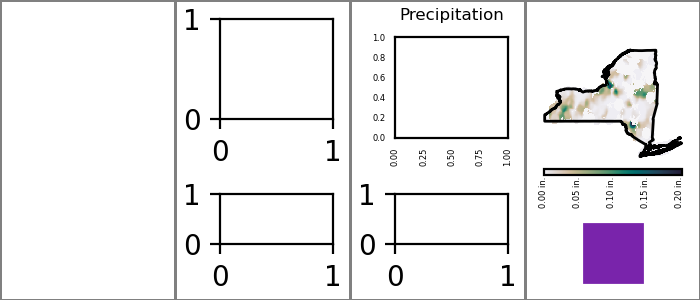
\includegraphics[width=1\columnwidth]{k_different_types.png}
  \caption{
  A a topological representation of the data (in purple) is a simplified representation of a view of how the records in a dataset are connected. The table can be viewed as a set of independent records; therefore it has a 0D continuity represented by the disconnected dots. These weather records are also samples of continuous measurements at each location, which can be modeled as the time series measurements being samples on a 1d continuous interval and the geospatial station measurements as sparse samples on a 2D continuous space. 
  \label{fig:related-work:continuity:ktypes}}
\end{figure}

There is an assumption in visualization that the connectivity of the elements in a dataset are preserved in the visual representation; roughly topology provides a method for encoding this connectivity \cite{wilkinsonGrammarGraphics2005}. Bertin gives the examples of discrete data values should be represented by discrete entities such as points, quantitive continuous data by lines, and surfaces through area marks \cite{bertinSemiologyGraphicsDiagrams2011a}. In \autoref{fig:related-work:continuity:ktypes} the records of the GHCN\cite{lawrimoreGlobalHistoricalClimatology2011} weather station table can be considered disconnected from each other and therefore have a 0D continuity. This means each distinct row can be reduced to a discrete point and it is expected  that each rows will be encoded as a discrete visual element, such as a standalone scatter point. Each station can also be considered a time series of weather observation since temperature and pressure are sampled from a 1D continuous measurement space. The connectivity of these observations can be modeled as an interval and the data is encoded as a line since that visual element is also 1D continuous. The measurements at set of stations on any given day is a sparse sampling of a 2D geospatial grid and the connectivity can be modeled as a 2D plane. Instead of interpolation, which is how continuity was preserved in the timeseries plot, in this instance the connectivity is preserved by plotting the stations in the map such that their relative distances are preserved. Encoding connectivity using the formalism of topological spaces allows us to encode the connectivity of the data in a uniform manner such that we can then generalize the preservation of that connectivity in the visual representation rather than constructing a condition specifically for each type of topology.

Visual algorithms assume the topology of their input data, as described in taxonomies of visualization algorithms Chi and by Troy and M\"{o}ller \cite{chiTaxonomyVisualizationTechniques2000,toryRethinkingVisualizationHighlevel2004}. For example, a \texttt{line} algorithm often does not have a way to query whether a list of (x,y) coordinates is the distinct rows, the time series, or the list of stations in \autoref{fig:related-work:continuity:ktypes}. While plotting the time series as a continuous line would be correct, it would be incorrect for a visualization to indicate that the distinct rows or stations are connected in a 1D continuous manner. Since topological continuity is generalizable, we propose the construction of topology types such that data can explicitly state its topology type and visual algorithms can check that this type matches their assumptions. The typing system proposed in this paper builds on Butler's proposal of using a mathematical structure called fiber bundles as an abstract data representation in visualization \cite{butlerVectorBundleClassesForm1992, butlerVisualizationModelBased1989}. We sketch out fiber bundles in \autoref{sec:atct:fiber-bundles}, but his work provides a thorough introduction to bundles for visualization practitioners. 

\subsection{Data Field Structure}
\label{sec:related-work:equivariance}
Along with preserving topology, visualization algorithms are expected to preserve the structure of the data fields, i.e. the column types in a table, when they translate data to visual representations. The mathematical term for this is equivariance and an equivariant map is a map that transforms input with structure to output with compatible structure. Bertin codified the idea that visual encoding of a data field should match the structure of the field; for example ordered data should be encoded as an ordered visual element or quantitative data as a quantitative visual element \cite{bertinSemiologyGraphicsDiagrams2011a}. This structure mapping is necessary to ensure that the visual representations in graphs are not distorting the data\cite{tufteVisualDisplayQuantitative2001} and graphs are easier to understand when properties match \cite{norman_things_smart}. The expectation of matching structure is generalized as a mapping of a binary operator that acts on the data domain to a binary operator that acts on the graphic domain by Mackinlay\cite{mackinlayAutomaticDesignGraphical1987}. An invertible binary operator is the basis of Kindlemannn and Scheideggers's algebraic model of visualization\cite{kindlmannAlgebraicProcessVisualization2014}. They propose three specific types of equivariance: that the visualization should not change if the data representation (i.e. the data container) changes, that data maps unambiguously to visual elements \cite{ziemkiewiczEmbeddingInformationVisualization2009}, that changing the data should correspond to changes in the visualization in a perceptually significant manner. In \autoref{sec:atct:sheaves} we introduce a uniform abstract data representation layer, the expectation of unambiguous mappings is expressed in \autoref{sec:atct:xi}, and the definition of equivariance introduced in \autoref{sec:artist:equivariance} includes the correspondence between data and visual changes. In this work, we formally specify the conditions necessary to build structure preserving components using category theory, because it provides a rich language for expressing the structure of objects, functions between objects, and the constraints that must hold for these functions to compose \cite{wielsManagementEvolvingSpecifications1998,yorgeyMonoidsThemeVariations}. A brief visualization oriented introduction to category theory is in Vickers et al \cite{vickersUnderstandingVisualizationFormal2013}, but they are applying category theory to semantic concerns about visualization design rather than library architecture. 

\subsection{Structure Preservation In Software}
\label{sec:related-work:software}
Visualization libraries are in part measured by how expressive the components of the library are, where expressiveness is a measure of which structure preserving mappings a tool can implement \cite{mackinlayAutomaticDesignGraphical1987}. While some visualization tools aim to automate the pairing of data with structure preserving visual representations, such as Tableau\cite{StoltePolaris2002,hanrahanVizQL2006,MackinlayShowme2007}, many visualization libraries leave that choice to the user. Libraries that provide small buildable components \cite{wongsuphasawatNavigatingWideWorld2021}, such as components for making boxes or translating data values to colors, mostly embed their connectivity assumptions in their visual algorithms and allow the user choose almost any component, regardless of structure preservation. Domain specific libraries are designed with the assumption of continuities that are common in the domain \cite{HeerSoftware2006}, and therefore can somewhat restrict the space of choices to algorithms that are appropriate for the data. 
Buildable component libraries such as matplotlib\cite{hunterMatplotlib2DGraphics2007} and D3\cite{bostockDataDrivenDocuments2011} support a wide variety of data types, but at the cost of visual algorithms with  parameters that are tuned to the expected data in a way that leaves the over all library feeling uncohesive. VTK\cite{hanwellVisualizationToolkitVTK2015,geveciVTK2012} provides a language for expressing the topological properties of the data, but does so in a non-uniform manner. On the other hand, the topology of a table as a set of discrete rows, as illustrated in \autoref{fig:related-work:continuity:ktypes}, is assumed by 
A Presentation Tool\cite{mackinlayAutomatingDesignGraphical1986, mackinlayAutomatingDesignGraphical1986} and grammar of graphics\cite{wilkinsonGrammarGraphics2005} and the ggplot\cite{wickhamGgplot2ElegantGraphics2016a}, vega\cite{satyanarayanDeclarativeInteractionDesign2014}, and altair\cite{vanderplasAltairInteractiveStatistical2018} libraries built on these frameworks. Image libraries such as Napari\cite{nicholas_sofroniew_2021_4533308} and ImageJ\cite{schneiderNIHImageImageJ2012} and its humanaties data ImagePlot\cite{studiesCulturevisImageplot2021} plugin assumed that the input is 2D continuous. Networking libraries such as gephi\cite{bastianGephiOpenSource2009} and networkx\cite{HagbergExploringNetwork2008} assume a graph like structure. These domain specific libraries tend to benefit from more cohesive apis, but at the cost of a much more limited set of visualization algorithms than the building block libraries. 


\section{Formal Properties of Data \& Graphics}
\label{sec:atct}
In this section, we propose a mathematical abstraction of the data input and graphic prerendered output. This mathematical abstraction has a robust language for expressing topology and fields; expresses how to verify that data continuity is preserved on subset, distributed, and streaming data representations; and formalizes the expectation of a correspondence between data and visual elements. 

\subsection{Uniform Abstract Data Representation}
\label{sec:atct:fiber-bundles}
We model data using a mathematical representation of data that can encode topological properties, field types, and data values in a uniform manner using a structure from algebraic topology called a fiber bundle. We extend Butler's proposal of bundles as abstract visualization data type \cite{butlerVectorBundleClassesForm1992,butlerVisualizationModelBased1989} by incorporating Spivak's methodology for encoding named data types from his fiber bundle representation of relational databases \cite{spivakDatabasesAreCategories2010, spivakSIMPLICIALDATABASES}. We build on this work to describe how to encode the connectivity of the data as a topological space, separately encode the fields as their own topological space with a typing system, and express the mappings between these two spaces.

\begin{definition} A \textbf{fiber bundle} $(\dtotalc, \dbasec, \pi, \dfiberc)$ is a structure with topological spaces $\dtotalc, \dfiberc, \dbasec$ and continuous surjective map $\pi: \dtotalc \rightarrow \dbasec$ \cite{FiberBundle2020,spanier1989algebraic}. 
\begin{equation}
  \label{eq:atct:fb:intro}
  \begin{tikzcd}[ampersand replacement=\&, row sep=huge]
   \dfiberc
    \arrow[r, hook, color=total] \& 
    \dtotalc
    \arrow[d, "\pi"',color=total] \\
     \& 
  \dbasec
     \arrow[u, "\dsectionc"', bend right, pos=.5, color=section, dashed]
  \end{tikzcd}
\end{equation} 
A map $\pi$ is a bundle projection map when 
\begin{enumerate}
  \item the \textcolor{fiber}{fiber space} \dfiberc\ is the preimage of the projection function $\pi$ at a point $\dbasepoint$ in the \textcolor{base}{base space} \dbasec\ such that $\dfiber_{\dbasepoint} = \pi^{-1}(\dbasepoint)$
  \item there is an open neighborhood $\openset_{\dbasepoint}$ surrounding each point in the base space $\dbasepoint \in \openset_{\dbasepoint} \subset \dbase$ such that the \textcolor{total}{total space} \dtotalc\ over the neighborhood is locally trivial $\dtotal\restriction_{\openset} = \openset \times \dfiber$
\end{enumerate}
\end{definition}
The first condition for a fiber bundle means that all points in a fiber space over a point in the base space map to the same base space point, which we rely on to establish that there is a formal binding between typed data value, discussed in \autoref{sec:atct:fiber:fiber} and the corresponding index, discussed in \autoref{sec:atct:fiber:base}. The condition of local triviality means that the fibers are identical over open neighborhoods and is what allows fiber bundles to be extremely generalizable, as discussed in \autoref{sec:atct:fiber:sections}
 
\begin{definition} A \textcolor{section}{\textbf{section}} $\dsectionc: \dbasec \rightarrow \dtotalc$ over a fiber bundle is a smooth right inverse of $\pi$ such that $\pi(\dsection(\dbasepoint)) = \dbasepoint$ for all $\dbasepoint \in \dbase$
\end{definition}
In \autoref{sec:atct:fiber:sections}, we propose that modeling data as sections provides a way to encapsulate topological and field structure in a uniform dimension and type independent manner. 

\subsubsection{Topological Structure: Base Space \dbase}
\autoref{sec:atct:fiber:base}
We encode the underlying connectivity of the data as the \textcolor{base}{base space} \dbase\ of the fiber bundle because it provides a uniform language for describing the topology regardless of how the data is subset. The base space \dbase\ is a topological space $(\dbase,\mathcal{T}_{\dbase})$, which means it  consists of the set of points ${\dbasepoint \in \dbase}$ and topology $\mathcal{T}_{\dbase}$ \cite{munkresElementsAlgebraicTopology1984}. The set \dbase\ is equipped with open subsets \openset, which are a generalization of an open interval. This means opensets contain points inside a bounded region on the topological space and excludes the points on the boundary \cite{TopologyVsTopology}. An openset that surrounds a point \dbasepoint\ is called an open neighborhood $\openset_{\dbasepoint}$. Opensets are key to constructing topologies, and are used in this paper to model subsets of the data contextualized within the larger continuity those subsets belong to. 

\begin{definition}
A \textbf{topology} $\mathcal{T}_{\dbase}$ on a space \dbase\ is a collection of open sets \openset\ of \dbase\ that satisfy the properties 
  \begin{itemize}
    \item the empty set $\varnothing$ and $\dbase$ are in $\mathcal{T}_{\dbase}$
    \item for all $\openset_i, \openset_j \in \mathcal{T}_{\dbase}$, the intersection $\openset_i \cap \openset_j$  is in $ \mathcal{T}_{\dbase}$
    \item for all $\openset_i, \openset_j \in \mathcal{T}_{\dbase}$, the union $\openset_i \cup \openset_j$ is in $ \mathcal{T}_{\dbase}$
  \end{itemize}
  such that the the topology provides an axiomatic way to construct the topological space $\dbase \coloneqq (\dbase,\mathcal{T}_{\dbase})$\cite{bradleyTopologyCategoricalApproach2020}.
\end{definition}
 A property of the base space \dbase\ of a fiber bundle is that it is a quotient topology, which  means that it contains the largest possible collection of distinct opensets, meaning each openset is as small as possible, of $\dbase$ that still preserve the underlying continuity of \dbase \cite{QuotientSpaceTopology2020}. For our purposes, $\dbase$ is a set of points that encodes the underlying connectivity of the our dataset, for example, $\dbase$ could be the discrete points, interval, or plane in \autoref{fig:related-work:continuity:ktypes}. We express the allowable ways to subset and compose points such that the connectivity is preserved as the topology $\mathcal{T}_{\dbase}$ on the data continuity. 

The topological structure of the data can be expressed programmatically by constructing data types that encapsulate the class of topological structure-.i.e point, line, plane, network, etc. We propose that these data types can be formally specified as objects of a category. 
\begin{definition} 
   An arbitrary \textbf{category} $\mathcal{C}$ consists of the following \textit{data}: 
\begin{enumerate}
  \item \textit{object}: X
  \item \textit{identity morphism}: $X \xrightarrow {id_x} X$
  \item \textit{morphisms}: $X \xrightarrow{f} Y$ between objects X, Y in $\mathcal{C}$
  \item \textit{composite morphism}: given the morphisms $X \xrightarrow{f} Y$ and $Y \xrightarrow{g} Z$, there exists a morphism $X \xrightarrow{g\circ f} Z$
\end{enumerate}
The data must satisfy the following \textit{rules}
\begin{enumerate}
  \item \textit{unitality:} for every morphism $ X \xrightarrow{f} Y$, there exists identity morphisms $id_x, id_y$ such that $f \circ id_x = f = id_y \circ f$
  \item \textit{associativity:} if any three morphisms $f, g, h$ are composable, 
    \begin{equation*}
      \begin{tikzcd}
        X \arrow[r, "f"] \arrow[rrr, "h\circ(g\circ f) = (h\circ g)\circ f"', bend right, dashed] & Y  \arrow[r, "g"] & Z \arrow[r, "h"] & W
        \end{tikzcd}}
  \end{equation*}
  then they are associative such that $h\circ(g\circ f) = (h \circ g) \circ f$  \cite{lawvere2009conceptual,riehlCategoryTheoryContext,maclaneCategoriesWorkingMathematician2013,fongInvitationAppliedCategory2019}. 
  \end{enumerate}
\end{definition}

We construct a base space category $\mathcal{\dbasec}$ to encapsulate the topological structure of the data. The category $\mathcal{\dbase}$ has open set objects $\opensetc$ and inclusion morphisms $\opensetc_i \xrightarrow{\iota} \opensetc_j$ such that $\opensetc_i \subseteq \opensetc_j$. The composability property expresses that inclusion is transitive, while associativity expresses that the inclusion functions can be curried in various equivalent groupings. By formally specifying the properties of the topological structure datatypes as $\mathcal{\dbase}$, we can express that these are the properties that are required as part of the implementation of the data type objects.  


\subsubsection{Data Fields: Fiber Space \dfiber}
\autoref{sec:atct:fb:fiber}
As mentioned in \autoref{sec:related-work:equivariance}, equivariance is traditionally evaluated as the preservation of field structure, which is based on the field type. To have a rich language for expressing field type, we generalize Spivak's fiber bundle formulation of table \cite{spivakDatabasesAreCategories2010,spivakSIMPLICIALDATABASES}. 

\begin{definition} A \textbf{type specification} is the bundle map $\pi: \mathscr{U} \rightarrow \textbf{DT}$. The base space $\textbf{DT}$ is the set of data types, and the total space $\mathscr{U}$ is the set of domains of those data types. Given an arbitrary data type $T \in \textbf{DT}$, the preimage $\pi^{-1} \subset \mathscr{U}$ is the domain of $T$ and $x \in \pi^{-1}(T)$ is an object of type $T$.  
\end{definition}
For example, if $T=\texttt{int}$, then the image $\pi^{-1}(\texttt{int}) = \mathbb{Z} \subset \mathscr{U}$ is the set of all integers. The domain $\mathscr{U}_{{\sigma}}$ is also a topological space, meaning there is no restriction on the dimensionality of the field, thus allowing for the encoding of multi-dimensional fields in the same manner as single dimensional fields. Since many fields can have the same datatype, Spivak formally defines a mapping from field name to field data type, akin to a  data base schema \cite{ullmanFirstCourseDatabase2008}. 
\begin{definition} A \textbf{schema} consists of a pair $(\fnames, \sigma)$ where $\fnames$ is the set of field names and $\sigma: \fnames \rightarrow \textbf{DT}$ is a function from field name to field data type. 
\end{definition}
The function $\sigma$ is composed with $\pi$ such that the bundle  $\pi_{\sigma}:\mathscr{U}_{\sigma} \rightarrow \fnames$ associates a field name $c \in C$ with the corresponding data type domain. Spivak then defines data records as sections on the bundle defined by $\pi_{\sigma}$. 
\begin{definition} A \textbf{record} is a function $\delement: \fnames \rightarrow \mathscr{U}_{\sigma}$ and the set of records on $\pi_{\sigma}$ is denoted $\Gamma^{\pi}(\sigma)$. Records must return an object of type $\sigma(\fname) \in \textbf{DT}$ for each field $c \in C$.
\end{definition}
Spivak then constructs tables as sections $\dsection: \dbase \rightarrow \Gamma^{\pi}(\sigma)$ from a key space $\dspace$ to the set of records $\Gamma^{\pi}(\sigma)$ on the schema bundle. Generalizing Spivak's formulation of tables, we define the fiber space in this work as the set of record functions 
\begin{equation}
  \dfiberc \coloneqq \{\delement: \fnames \rightarrow \mathscr{U}_{\sigma} \bigm{\vert} \pi_{\sigma}(\delement(\fname)) = \fname\;for\;all\; \fname \in \fnames \}
\end{equation}
such that the preimage of a point is the corresponding data type domain $\pi^{-1}(\dbasepoint) = \dfiber_{k} = \mathscr{U}_{{\sigma}_{\dbasepoint}}$. The construction of the fiber as the space of records provides a way to distinguish data fields with the same datatype while allowing that datatype to be defined as almost any arbitrary topological space. 

As with the base space category $\mathcal{\dbase}$, we propose a fiber category $\mathcal{\dfiberc}$ to encapsulate the field types of the data. The fiber category $\mathcal{\dfiberc}$ is a monoidal category, meaning the category has a single object $\dfiberc$ of an arbitrary type. The morphisms on the fiber object are $\dfunctc \in Hom(\dfiberc, \dfiberc)$. The fiber category is equipped with a bifunctor $\otimes: \mathcal{\dfiber} \times \mathcal{\dfiber} \rightarrow \mathcal{\dfiber}$. The bifunctor provides a method for combining fibers, thereby allowing for fields that contain multityped values. For example, wind can be represented as two fields $\dfiber_{speed} \times \dfiber_{direction}$ or a composite fiber field $\dfiber_{speed} \otimes \dfiber_{direction} = \dfiber_{wind}$. The $\otimes$ encapsulates both the sets associated with each fiber $\mathbb{R} \times \mathbb{R} = \mathbb{R}^{2}$ and the morphisms associated with each functor $(\dfunct_{speed}, \dfunct_{direction}) = \dfunct_{wind}$. Defining the field schema as a monoidal category allows us to formally express the structure of the field, as defined by its sets and functions, at different levels of composition as needed by different visualization tasks.
 

\subsubsection{Data: Section \dsection} 
\autoref{sec:atct:fb:sections}
We encode data as a \textcolor{section}{section} \dsectionc\ of a bundle because this allows us to incorporate the topology and field types in the data definition. We can define these section functions locally, meaning over a specific open subset \openset\ of \dbase\ 
\begin{equation}
  \label{eq:atct:fb:sections}
  \cgamma{\opensetc}{\dtotalc\restriction_{\opensetc}} \coloneqq \big\{\dsectionc: \opensetc\rightarrow \dtotalc\restriction_{\opensetc} \; \bigm{\vert} \pi(\dsectionc(\dbasepointc)) = \dbasepointc\;for\, all\; \dbasepointc \in \opensetc \big\} 
\end{equation}
such that each section function $\dsection: \dbasepoint \mapsto \delement$ maps from a point $\dbasepoint \in \openset$ to a record in the fiber space $\delement \in \dfiber_{\dbasepoint}$ over that point. Bundles can have multiple sections, as denoted by $\Gamma(\openset, \dtotal\restriction{\openset})$. We can therefore model data as structures that map from an index like point $\dbasepoint$ to a data record $\delement$, and encapsulate multiple datasets with the same fiber and base space as different sections of the same bundle. 

In a trivial bundle all fibers are equal $\dfiberc \equiv \dfiberc_{\dbasepointc}\;\forall \dbasepointc \in \dbase$, which means that $\dtotalc = \dbasec \times \dfiberc$ . This allows us to define global sections $\dsection: \dbase \rightarrow \dfiber \in \Gamma(\dbase, \dfiber)$ which we translate into a data signature of the form  
\begin{equation}
  \textcolor{section}{\texttt{dataset}}: \textcolor{base}{\texttt{topology}} \rightarrow \textcolor{fiber}{\texttt{field}}
\end{equation}
where $\dsection=\texttt{dataset}$, $\dbase=\texttt{topology}$ and $\dfiber=\texttt{fields}$. This type signature provides a method of explicitly stating the topology and field type of the data and generalizes to almost any topology and fiber type, provided that the total space is trivial. 

When the total space is non-trivial, we can use the fiber bundle property of local-triviality to generate type signatures. In a non-trivial bundle, fibers are isomorphic $\dfiber \simeq \dfiber_{\dbasepoint}\;\forall \dbasepoint \in \dbase$, which means there is no single fiber type $\dfiber$. Instead, we can define sections locally $\dsection\restriction_{\openset} \in \Gamma(\openset_{\dbasepoint}, \dtotal\restriction_{\openset_{\dbasepoint}})$, which means a section defined only on an open neighborhood $\dbasepoint \in \openset \in \dbase$. This is because all fiber bundles are locally trivializable, $\dtotal\restriction_{\openset_{k}} = \openset_{k}\times \dfiber$ such that there's always a subset where the fibers are equal. This means almost all data can be expressed as a collection of local sections $\{\dsection\restriction_{\openset_{\dbasepoint}}| \dbasepoint \in \dbase \}$ which translate to a set of signatures 
\begin{equation}
  \begin{split}
\{\textcolor{section}{\texttt{data-subset}}: \textcolor{base}{\texttt{topology}} \rightarrow \textcolor{fiber}{\texttt{fields}} \\
 s.\;t.\;\textcolor{section}{\texttt{data-subset}} \in \texttt{dataset}\}  
  \end{split}
\end{equation}
that can be glued together on overlaps to generate the dataset. This gluing can be implemented as part of the data container, which we discuss in \autoref{sec:atct:sheaves}.


\subsubsection{Examples}
\begin{figure}[h!]
  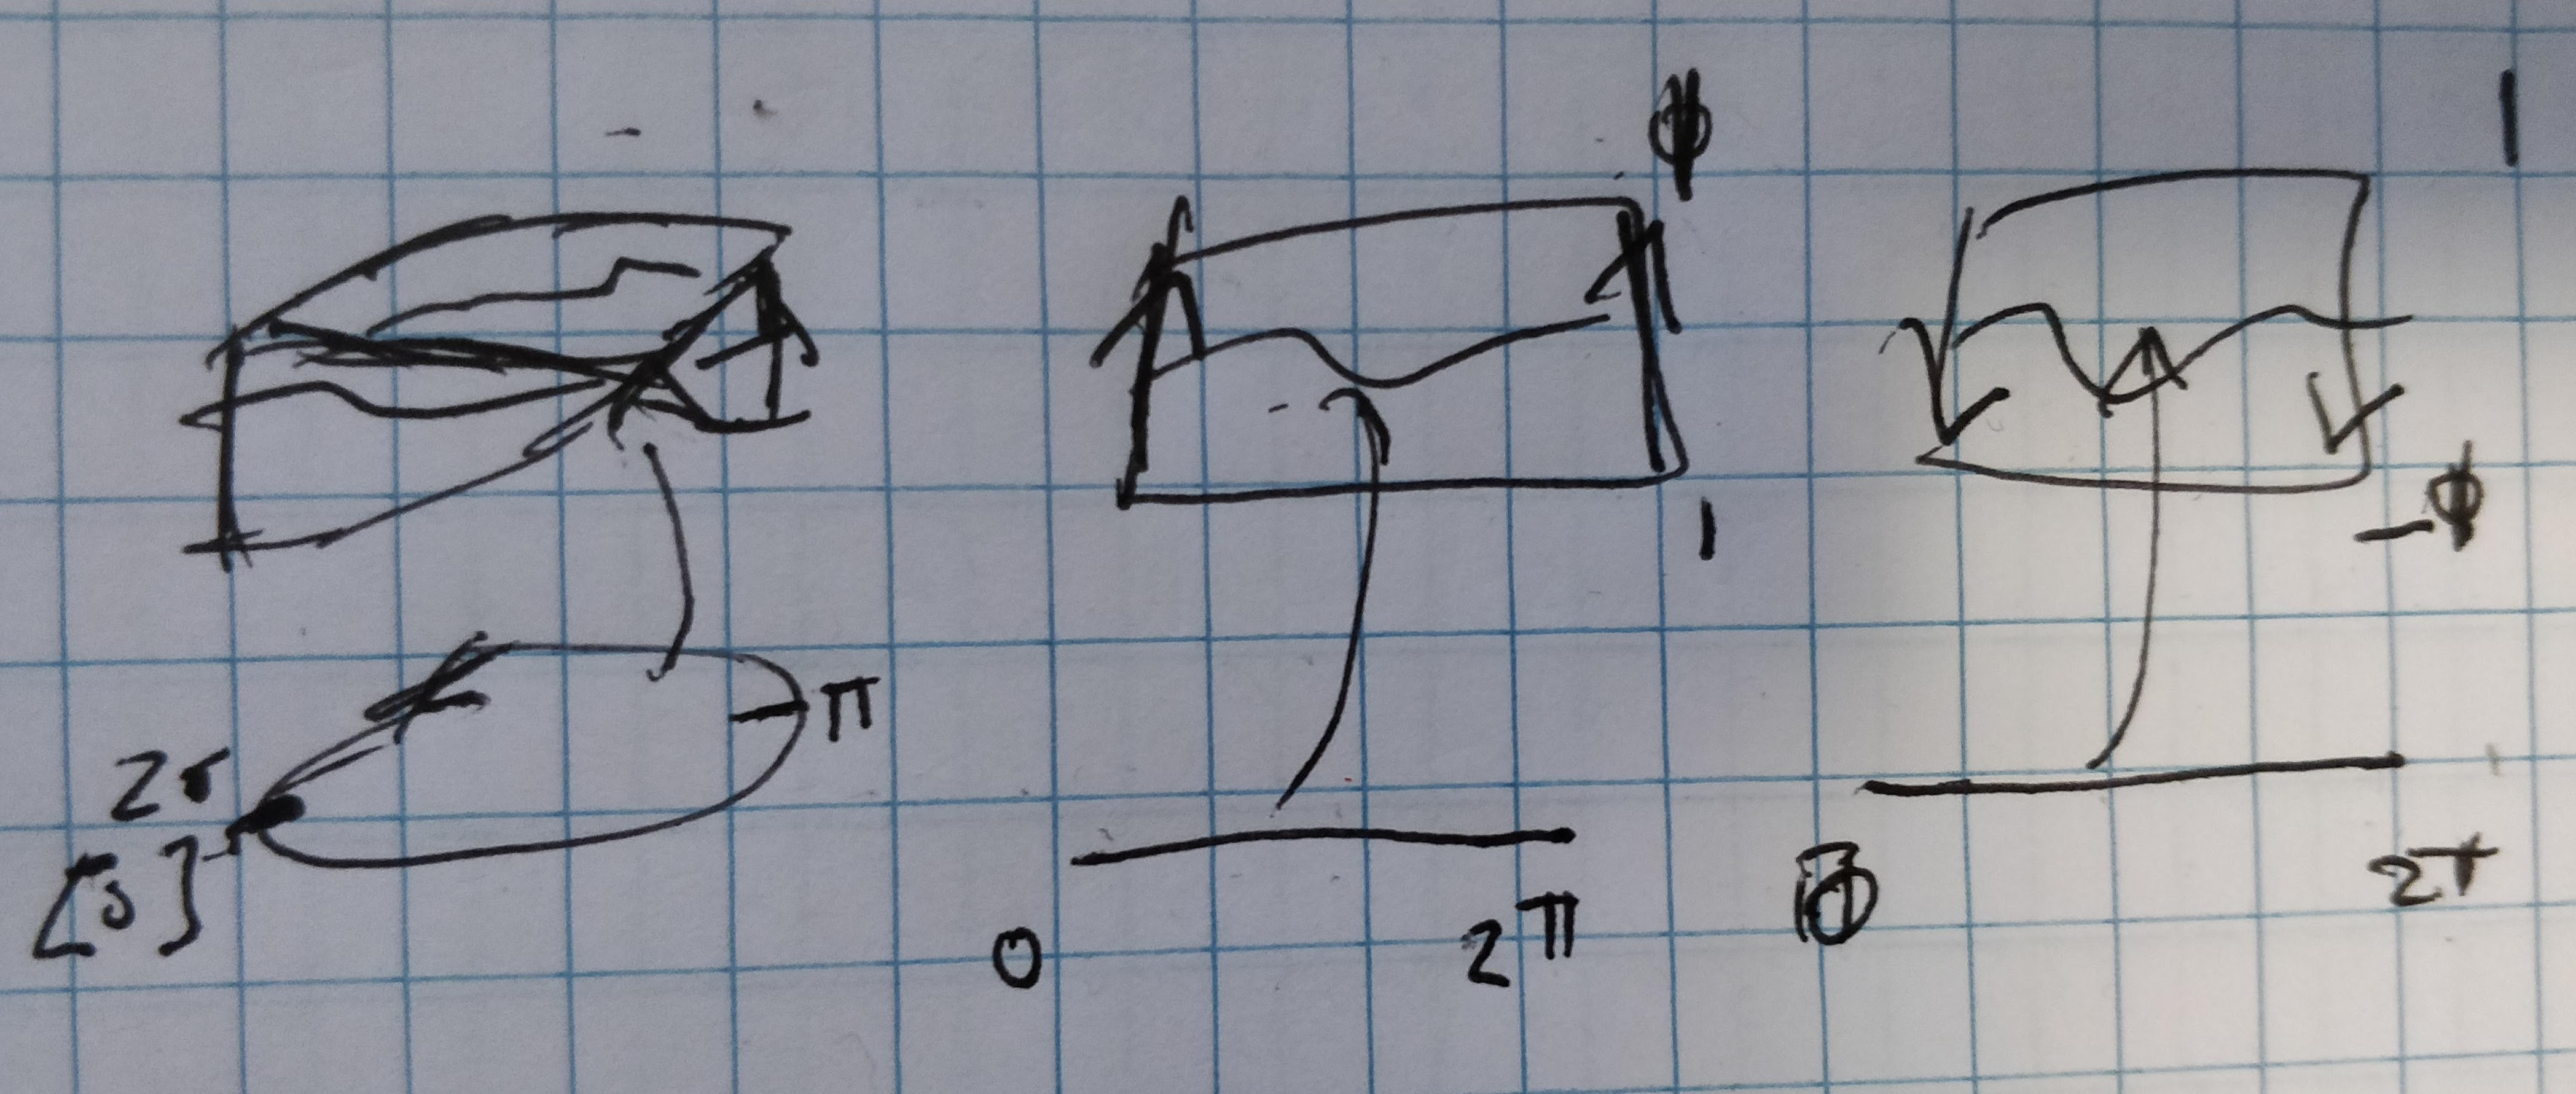
\includegraphics[width=\columnwidth]{tbundle.png}
  \caption{The mobius band is a non-trivial total space because the twist means that the fibers are sometimes [-1, 1] and other times [1,-1]. The mobius band can be represented as two trivial bundles, one with fiber [-1,1] and one with fiber [1,-1] that can be glued on the edges into the band. The gluing rules ensure that the arrows on the edges go in the same direction.\label{fig:atct:nontrivialbundle}}
\end{figure}

The mobius band is an example of the non-trivial bundle because the twist in the middle means that the fibers are not the same, as shown in \autoref{fig:atct:nontrivialbundle}. But, as with all bundles, the mobius band can be decomposed into trivial bundle components, here the two sides of the mobius band. Each side has fibers going in the same direction, with the mismatch only apparent on the edges. These trivial bundles can be glued into the mobius band so long as the fibers (arrows on the edges) go in the same direction when glued. The data is encoded as the section of the bundle, here the sin curve. 

\begin{figure}[h!]
  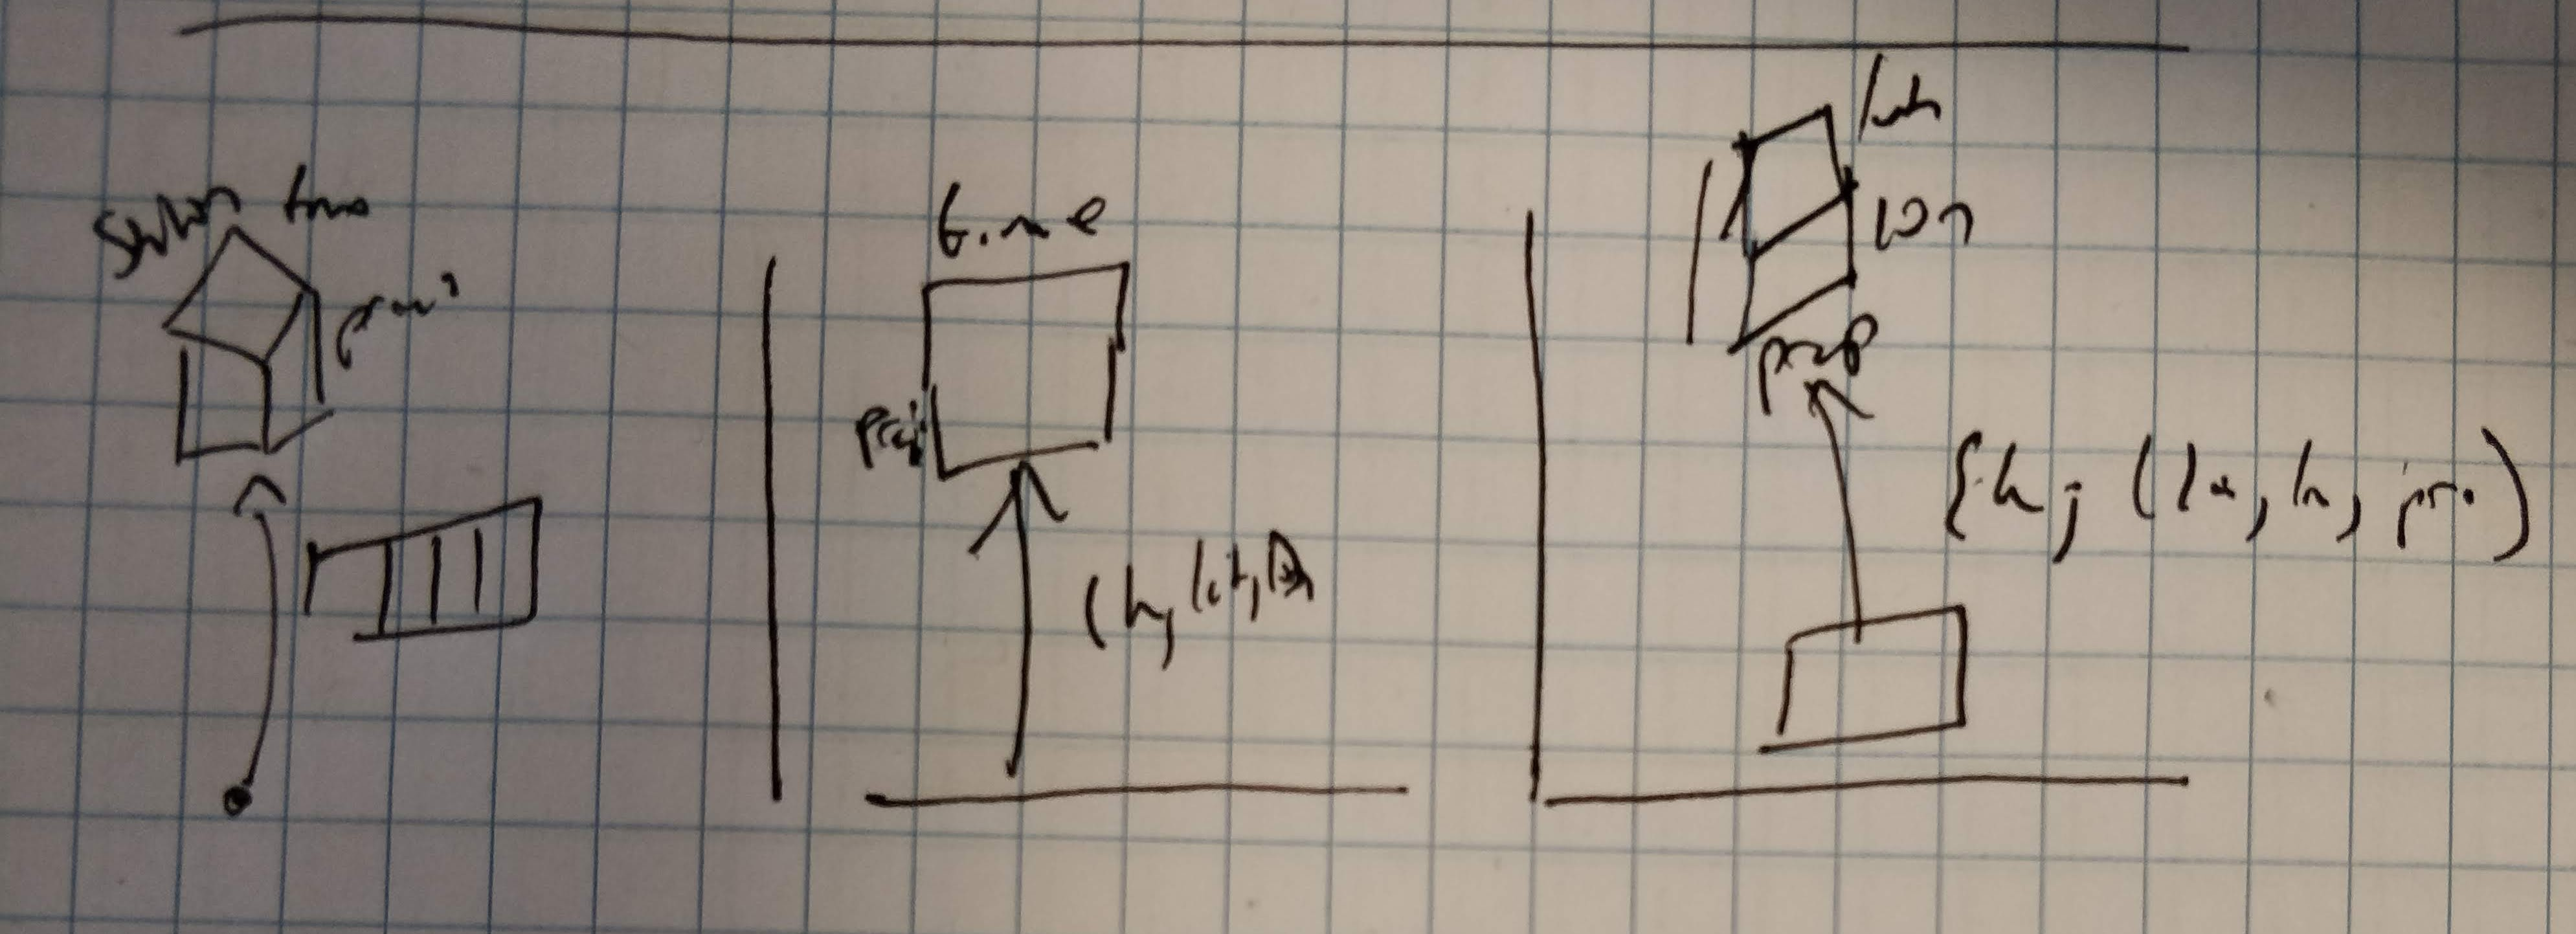
\includegraphics[width=\columnwidth]{dbundle.png}
  \caption{The table from \autoref{fig:related-work:continuity:ktypes} has a 3 dimensional fiber (name, temperature, precipitation), a 0D base space, and the row is the section. The time series has a 2D fiber (time, precipitation) and a 1D base space since the data is sampled along a continuous space (physical time). Each section returns a data point along the line. The map is sparsely sampled points along a 2D plane encoding spatial continuity, and the fiber is a 3D space encoding (latitude, longitude, precipitation)
    \label{fig:atct:trivialbundle}}
\end{figure}

In \autoref{fig:atct:trivialbundle}, the base space $\dbase$ acts as an indexing space into the fiber space $\dfiber$. In the bundle encoding of the table, the indexing space is random keys; in the time series bundle, the base space is the interval [0,1]; and the map is sparse samples from a continuous space $[0,1]^{2}$ In contrast to a notion of a semantic binding between indexing space and field values, as proposed by Munzner\cite{munznerVisualizationAnalysisDesign2014}, the fields describing the continuity are part of the fiber. For example, the time is a fiber in the timeseries and the latitude and longitude are part of the map's fiber. This separation between connectivity and what it is called means the time or location can change units without a change to structure. It also provides a way to express data that may seem continuous but isn't, for example independent measurements over time. The data in \autoref{fig:atct:trivialbundle} comes from the same dataset; therefore we know that the bundles share connectivity and fiber space. It is expected that shared components be translated to visual elements in a consistent manner \cite{hullmanKeeping2018}, and in \autoref{sec:artist:operators} we introduce operators for expressing which components are shared and how to verify that they have been mapped into visual elements in a consistent manner. 

\subsubsection{Uniform Abstract Graphic Representation}
One of the advantages of fiber bundles is that they are general enough that we can also encode the output of a visual algorithm as a bundle. This allows us to use the same structure to express the properties of data and the graphic that must be symmetric to the data in an equivariant (\autoref{sec:related-work:equivariance}) transformation. We denote the output as a graphic, but the use of bundles allows us to generalize to output on any display space, such as a screen or 3D print. 
\begin{equation}
  \label{eq:atct:fb:graphic}
  \gfiberc \hookrightarrow \gtotalc \xrightarrow{\pi} \gbasec
\end{equation}
The total space \gtotalc\ is an abstraction of an ideal (infinite resolution) space into which the graphic can be rendered. The base space \gbasec\ is a parameterization of the display area, for example the inked bounding box in cairo \cite{CairographicsOrg}. The fiber space \gfiberc\ is an abstraction of the renderer fields, for example $\{x,\,y,\,r,\,g,\,b,\,a\}$. 

As with data, we model the graphic generating functions as sections $\gsection$ of the graphic bundle 
\begin{equation}
  \label{eq:atct:fb_graphic_section}
  \cgamma{\opensetgc}{\gtotalc\restriction_{\opensetgc}} \coloneqq \big\{\gsectionc: \opensetgc\rightarrow \gtotalc\restriction_{\opensetgc} \; \bigm{\vert} \pi(\gsectionc(\gbasepointc)) = \gbasepointc\;for\, all\; \gbasepointc \in \opensetgc \big\}
\end{equation}
that map from a point in an openset in the graphic space $\gbasepoint \in \opensetg \in \gbase$ to a point in the graphic fiber $\gfiber$. The section evaluated on a single point $\gbasepoint$ returns a single graphic record, for example one pixel in an ideal resolution space. In our model, the unevaluated graphic section is passed to a renderer to generate graphics. 

\begin{figure}[h!]
  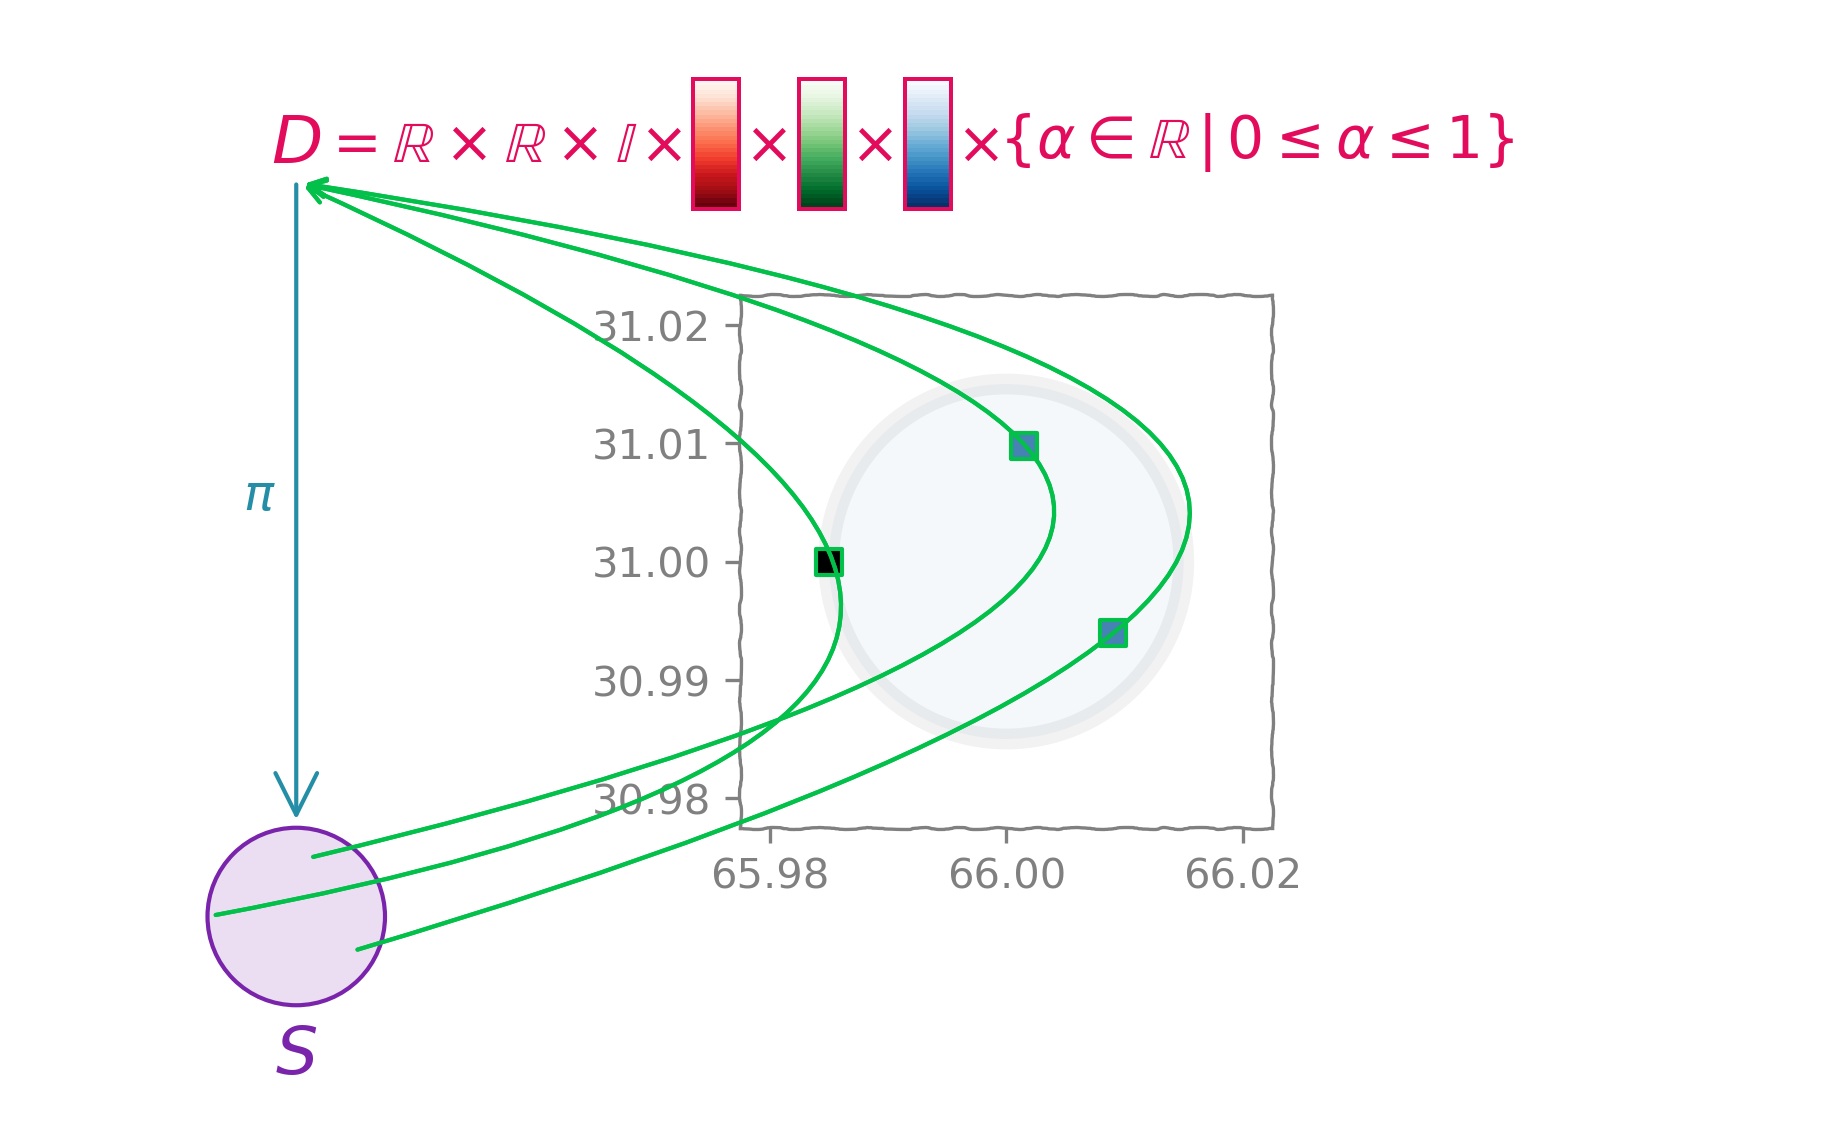
\includegraphics[width=1\columnwidth]{fb_rho.png}
  \caption{For a 2D display a section $\gsection$ maps from each point $\gbasepoint$ into a fiber $\gfiber_{\gbasepoint}$ that encodes an RGB prerender space with infinite resolution $\mathcal{R}^{2}$. Each tiny colored box is an approximation of the return value of the same section function $\gsection$ evaluated on different points $\gbasepoint \in \gbase$ in the base space. We represent all $\gfiber_{\gbasepoint}$ as the fiber $\gfiber$ because a 2D bundle is a trivial bundle so $\gfiber_{\gbasepoint} = \gfiber$ for all \gbasepoint.
  \label{fig:atct:fb:graphic}}
\end{figure}

In \autoref{fig:atct:fb:graphic}, the section function $\gsection$ maps into the fiber for a simplified 2D RGB infinite resolution prerender space and returns the $\{x,y,r,g,b\}$ values of a pixel in an infinite resolution space. In \autoref{fig:atct:fb:graphic} these pixels are approximated as the small orange and black colored boxes. Each box is the output of the $\gsection(\gbasepoint)$ section that intersects the box. The set of all pixels returned by a section evaluated on a given visual base space $\gsection|_{\gbase}$ can yield a visual element, such as a marker, line, or piece of a glyph. \autoref{fig:atct:fb:graphic} illustrates a highly idealized space with no overlaps. To support overlaps, we can add another fiber element $\gfiber_{z}$ and leave it to the renderer to appropriately blend layers. 

\subsection{Formal Properties of Data Containers}
\label{sec:atct:sheaves}
Sheaves are a mathematical way to describe the expectation that data structures implement the bookkeeping that keeps track of the continuity of the data and graphic \cite{ghristElementaryAppliedTopology2014}. These constraints generalize to data that is subsetted, distributed, streaming, and on-demand. Sheaves are built out of presheaves, which are functors, meaning they are functions from objects of one category to objects of another category\cite{WhatFunctorDefinitions} that preserve the morphisms in each category. 
\begin{definition} A \textbf{functor} is map $F: \mathcal{C} \rightarrow \mathcal{D}$ such that every object $C \in \mathcal{OB(C)}$ has a corresponding object $F(C) \in \mathcal{OB(D)}$ in category $\mathcal{D}$. The functor also acts on morphisms such that for every morphism $f: C_1 \rightarrow C_2$ in category $\mathcal{C}$, there is a compatible morphism $F(f): F(C_{1}) \rightarrow F(C_2)$. 
A functor must satisfy the properties 
\begin{itemize}
  \item \textit{identity}: $F(id_{C}(C)) = id_{D}(F(C))$
  \item \textit{composition}:$F(g)\circ F(f) = F(g\circ f)$ for any composable morphisms $C_{1}\xrightarrow{f} C_2$, $C_2 \xrightarrow{g} C_3$
\end{itemize}
\end{definition}
Functors preserve all the structure of the categories, namely the domains, codomains, composition, and identities\cite{riehlCategoryTheoryContext}$. Specifically, functors allow us to express which structure must be preserved when an object is transformed from one category to another. 

The presheaf encodes the expectation that continuity is preserved across sections. Specifically, a presheaf is a contravariant functor from an object in an arbitrary category to an object in the category \setb\cite{nlab:presheaf}. 
\begin{equation}
  \label{eq:atct:sheaf:functor}
  \sheafc_{\dbasec, \dtotalc}: \opensetc \rightarrow \cgamma{\opensetc}{\dtotalc\restriction_{\opensetc}}
\end{equation}
The presheaf expresses that every subset of the data $\openset$ has an associated set of data sections $\cgamma{\opensetc}{\dtotalc\restriction_{\opensetc}}$. The presheaf is a contravariant functor because the morphisms between input objects
\begin{equation*}
  \iota: \openset_1 \rightarrow \openset_2
\end{equation*}
go in the opposite direction from the restriction morphisms $\iota^*$ between the sets
\begin{equation*}
  \iota^*: \cgamma{\openset_2}{\dtotal_{\openset_2}} \rightarrow \cgamma{\openset_1}{\dtotal_{\openset_1}}
\end{equation*}
which are the outputs of the sheaf $\sheaf(\openset) = \cgamma{\openset}{\dtotal\restriction_{\openset}}$. We use a presheaf to describe the expectation that any set of sections defined over a larger space $\dsection \in \Gamma(\opensetc_2, \dtotal\restriction_{\openset_{2}})$ is also defined over subspaces of that space $\dsection\restriction_{\opensetc_{1}}$. This means any data container must implement subsetting in a manner that  makes sense for the continuity, for example an appropriate interpolation for continuous data.

While the presheaf is a generalization of the concept of a global space of sections $\Gamma(\dbase, \dtotal)$ \cite{spanier1989algebraic}, the locality and gluing axioms \cite{bakerMathsSheaf} of a sheaf describe the conditions for verifying that the sections over subspaces are part of a cohesive section over the whole space. 
\begin{definition} A \textbf{sheaf} is a presheaf that satisfies the following two axioms
\begin{itemize}
  \item \textit{locality} two sections in a sheaf are equal $\dsection^{a} = \dsection^{b}$ when they evaluate to the same values over the same set of open sets $\dsection^{a}|{\openset} =  \dsection^{b}|_{\openset}$.
  \item \textit{gluing} the union of sections defined on specific open sets is equivalent to one big section over the union of spaces $\dsection|_{\openset_{i} \cup \openset_{j}} = \dsection^{i}|_{\openset_i} \cup \dsection^{j}|_{\openset_j}$ if these sections agree on overlaps $\dsection^{i}|_{\openset_i\cap\openset_j} =  \dsection^{j}|_{\openset_i\cap\openset_j}$
  \end{itemize}
\end{definition}
The gluing axiom says that a distributed representation of a dataset, which is a set of local sections, is equivalent to a section over the union of the opensets of the local sections. The locality axiom asserts that the glued section function is equivalent to a function over the union if they evaluate t the same values. The gluing axiom can also be used to generate the gluing rules used to construct non-trivial bundles from the set of trivial local section. Generally, the sheaf asserts the expectation that the data container is implemented such that the connectivity between the opensets (underlying data continuity) is preserved. 

Each section of a sheaf over a point returns a single record in the fiber. The sheaf over an open set $\openset$ surrounding a point $\dbasepoint$ is called a stalk\cite{StalkSheaf2019}
\begin{equation}
  \label{eq:atct:sheaf:stalk}
    \sheaf_{\dbase, \dtotalc}\restriction_{\dbasepoint}\coloneqq \lim\limits_{\openset\ni \dbasepoint} \Gamma(\openset, \dtotal\restriction_{\openset}) 
\end{equation}
where the fiber is contained inside the stalk  $\dfiber_{\dbasepoint} \subset  \sheaf_{\dbase, \dtotal}\restriction_{\dbasepoint}$. The germ is the section evaluated at a point in the stalk  $\dsection(\dbasepoint) \in \sheaf_{\dbase, \dtotal}\restriction_{\dbasepoint}$ and is the data. The stalk and germ in the stalk provide the derivative of the record, which is needed for some computational and visualization tasks. 

\subsection{Mathematical Structure of Data}
\label{sec:atct:sheaves:measurments}
\note{move to Artist }
Equivariance in a visual context was formally defined as the preservation of a binary operator from one domain to another by Mackinlay\cite{mackinlayAutomaticDesignGraphical1987}. We generalize binary operations to actions $\dfunc \in \dfuncset$ on elements of the bundle $\delement \in \dtotal$. This is expressed with a composition function  $act: \dfuncset \times E \rightarrow \dtotal$ that applies the action to an element of \dtotal\ such that $\dfunc(\delement_0) = \delement_1, \delement_0, \delement_1 \in \dfunc$. We generalize to a family of actions because that allows for expanding the set of allowable transformations on the data beyond a single operator. 

We separate data transformations into two components, transformations on the base space $(\dfunchc, \dfuncpullc)$ and transformations on the fiber space $\dfunctc$. These diagrams are separated because the base space transformation and the pullback are functors on the openset object and associated set of sections, while the fiber transformation takes a single fiber to a different fiber in the set of sections. 

\begin{equation}
  \label{eq:atct:sheaves:monoid_morphism}
  \begin{tikzcd}
    \cgamma{\opensetc}{\dtotalc\restriction_{\opensetc}} 
    \arrow[rr, "\dfuncpullc", color=action, maps to] &  & 
    \cgamma{\opensetc^{\prime}}{\dfuncpullc\dtotalc\restriction_{\opensetc^{\prime}}} & 
    \cgamma{\opensetc^{\prime}}{\dfuncpullc\dtotalc\restriction_{\opensetc^{\prime}}} 
    \arrow[dd, "\dfunctc", color=action] \\
     &  & &       \\
    \opensetc 
    \arrow[uu, maps to,color=sheaf]  &  & \opensetc^{\prime} 
    \arrow[ll, "\dfunchc"', color=action, maps to] 
    \arrow[uu, maps to, color=sheaf] & \cgamma{\opensetc^{\prime}}{\dfuncpullc\dtotalc\restriction_{\opensetc^{\prime}}}                       
    \end{tikzcd}
\end{equation}
As shown in \autoref{eq:atct:sheaves:monoid_morphism}, the base space transform 
\begin{equation}
 \label{eq:atct:morphism:base}
\dfunch: \openset^{\prime}\rightarrow \openset
\end{equation}
The base space transformation is from one open set to another open set in the same base space $\openset, \openset^{\prime} \subseteq \dbase$. To correctly align the sections with the remapped base space, there is a a corresponding section pullback function
\begin{equation}
  \label{eq:atct:morphism:basepull}
  \dfuncpull \dsection \restriction_{\openset^{\prime}}: \dsection\restriction_{\openset^{\prime}} \mapsto \dsection \restriction_{\openset^{\prime} \circ \dfunch} 
\end{equation}
such that $\dsection|_{\openset} = \dfuncpull\dsection|_{\opensetc^{\prime}}$ because $\dsection|_{\openset} = \dsection|_{\dfunch(\opensetc^{\prime})}$. This means that the base space transformation \dfunch\ does not change the data values at a given point
\begin{equation}
  \label{eq:atct:morphism:verify_base}
  \dsection(\dbase) = \dfuncpull\dsectionc(\dbasepoint^{\prime}) = \dsection(\dfunch(\dbase^{prime}))
\end{equation} 
where $\dfunch(\dbasepoint^{\prime}) = \dfunch(\dbasepoint)$. 
As introduced in \autoref{def:atct:io:fiber}, the fiber transformation $\dfunct: \dfuncpull \dtotal_{\dbasepoint^{\prime}} \rightarrow \dfuncpull \dtotal_{\dbasepoint^{\prime}}$ is a morphism on the fiber $\dfunct \in Hom(\dfuncpull\dfiber\restriction_{\dbasepoint^{\prime}},\dfuncpull\dfiber\restriction_{\dbasepoint^{\prime}})$ restricted to a point $\dbasepoint^{\prime} \in \openset^{\prime}$. The fiber transformation is a change in section 
\begin{equation}
  \label{eq:atct:morphism:fiber}
  \dfunct: \dfuncpull \dsection \restriction_{\openset^{\prime}} \mapsto \dfuncpull \dsection^{\prime} \restriction_{\openset}
\end{equation}
where $\dsection, \dsection^{\prime} \in \Gamma(\openset^{\prime}, \dfuncpull\dtotal\restriction_{\openset^{\prime}})$. Since there are many different fiber transformations,  there is not a uniform way of expressing how this morphism acts on sections unlike in \label{eq:atct:morphism:verify_base}. Examples of a fiber transformation are actions such as partial ordering for ranking purpose \cite{bruggemannRankingPrioritizationMultiindicator2011} and the permutation, ordering, translation, and scaling codified as Steven's measurement scales \cite{stevensTheoryScalesMeasurement1946m, leaFormalizationMeasurementScale, thomasMathematizationNotMeasurement2014}. 

We define a full data transformation as one that induces both a remapping of the index space and a change in the data values
\begin{equation}
  \label{eq:atct:morphism:all}
  \dfuncc: \dsectionc\restriction_{\opensetc} \mapsto \dsectionc^{\prime}\restriction_{\opensetc} \circ \dfunchc
\end{equation}
which gives us an equation that can express transformations that have both a base space change and a fiber change. 

The data transform \dfunc\ is composable 
\begin{equation}
  \dfuncc = (\dfunchc, \prod\limits_{i=0}^{n}\dfunctc_i)
\end{equation}
if each (identical) component base space is transformed in the same way $\dfunch$ and there exists functions $\dfunc_{a,b}: \dtotal_a \times \dtotal_b \rightarrow \dtotal_a \times \dtotal_b$, $\dfunc_{a}: \dtotal_a \rightarrow \dtotal_a$ and $\dfunc_{b}: \dtotal_b \rightarrow \dtotal_b$ such that $\pi_a \circ \dfunc_a = \dfunc_{a,b} \circ \pi_a$ and $\pi_b \circ \dfunc_b = \dfunc_{a,b} \circ \pi_b$ then $\dfunc_{a,b} = (\dfunc_a, \dfunc_b)$. This allows us to define a data transform where each fiber transform $\dfunct_{i}$ can be applied to a different fiber field $\dfiber_i$. 

\begin{figure}[h!]
  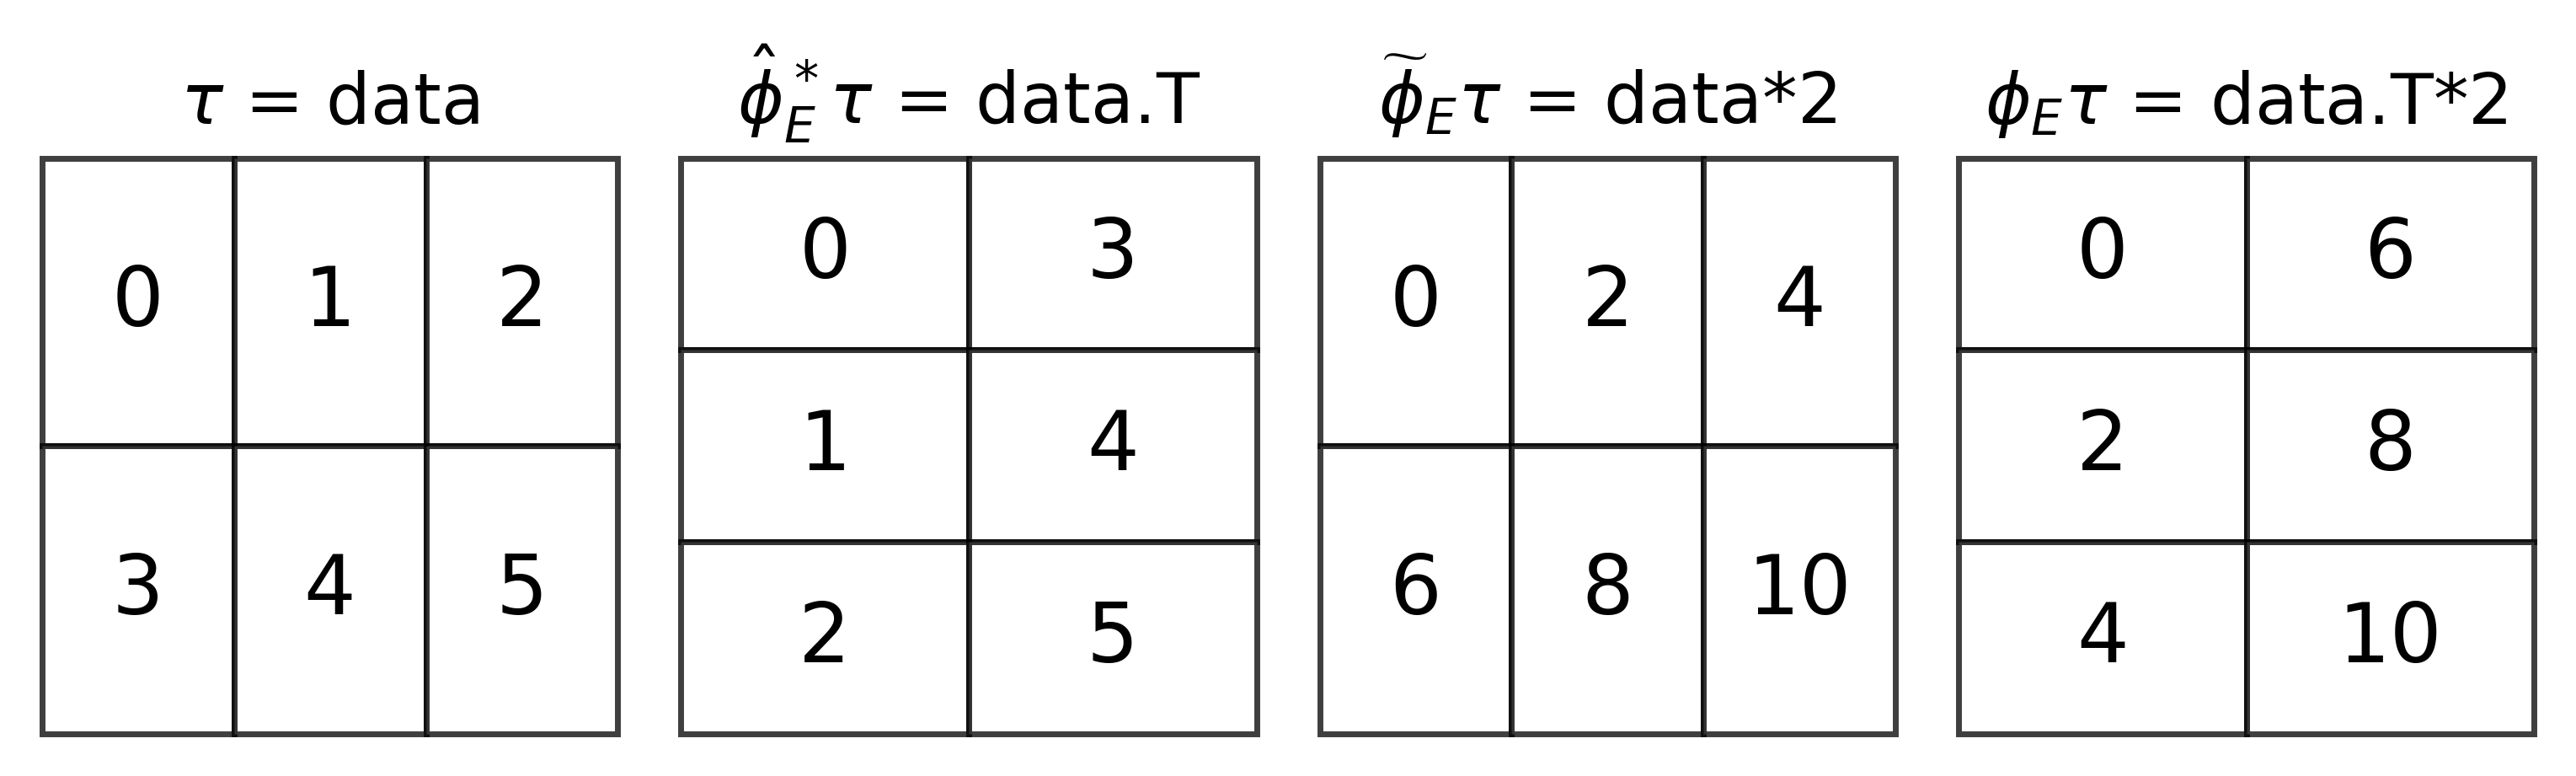
\includegraphics[width=\columnwidth]{phi.png}
  \caption{Values in a data set can be transformed in three ways: $\dfunch$-values can change position, .e.g transposed;  $\dfunct$-values can change, e.g. doubled; $\dfunc$ - values can change position and value  \label{fig:atct:phi}}
\end{figure}
\autoref{fig:atct:phi} provides an example of a transposition base space change \dfunch, a scaling fiber space change \dfunct, and a composition of the two \dfunc\ applied to each data point $x_{\dbasepoint} \in \texttt{data}$. In the transposition only case, the values in $\dfuncpull\dsection$ retain their neighbors from $\dsection$ because \dfunc\ does not change the continuity. Each value in $\dfuncpull\dsection$ is also the same as in $\dsection$, just moved to the new position. In $\dfunct\dsection$, each value is scaled by two but remains in the same location as in $\dsection$. And in $\dfunc\dsection$ each function is transposed such that it retains its neighbors and all values are scaled consistently. 

\subsection{Data and Graphic Correspondence}
\label{sec:atct:xi}
There is an expectation that for a visualization to readable, the visual elements must correspond to distinct data elements\cite{ziemkiewiczEmbeddingInformationVisualization2009} and we can use the properties of sheaves to formally express this correspondence. First we establish that the graphic continuity corresponds to the data continuity by proposing that there exists a continuous \textcolor{functor}{map between topological spaces} \vindexc 
\begin{equation}
  \label{eq:atct:xi}
  \vindexc: \opensetgc \rightarrow \opensetc 
\end{equation}
such that every $\opensetg \subseteq \gbase$ must map to a corresponding set $\openset \subset \dbase$. The functor $\vindex$ is surjective such that for every point $\dbasepoint \in \openset$ there is a corresponding set of points $\{\gbasepoint | \gbasepoint \in  \vindexpre(k)\}$ for all $\gbasepoint in \opensetg$.

Given the map between spaces \vindex\, a property of sheaves is that there exist image functors\cite{ImageFunctorsSheaves2021} functors \vindexpull\ and \vindexpush that can transport sheaves over other base spaces.
\note{insert formal def of pull back and pushforward functors}
The \textcolor{functor}{pullback functor} $\vindexpullc$ sends sheaves over $\dbase$ to $\gbase$ and the \textcolor{functor}{pushforward functor} $\vindexpushc$  sends sheaves over $\gbase$ to $\dbase$
\begin{equation}
  \label{eq:atct:morphisms:xi}
\begin{tikzcd}[row sep=huge]
  \cgamma{\opensetc}{\dtotalc\restriction_{\opensetc}} 
  \arrow[rr, "\vindexpullc", maps to, color=functor] &  & 
  \cgamma{\opensetgc}{\vindexpullc\dtotalc\restriction_{\opensetgc}}  \\
  \opensetc 
  \arrow[d, "{\vindexpushc\sheafc_{\gbasec,  \gtotalc}}", dashed, maps to, color=sheaf] 
  \arrow[u, "{\sheafc_{\dbasec, \dtotalc}}"', maps to, color=sheaf] &  & 
  \opensetgc 
  \arrow[d, "{\sheafc_{\gbasec, \gtotalc}}", maps to, color=sheaf] 
  \arrow[u, "{\vindexpullc\sheafc_{\dbasec, \dtotalc}}"', dashed, maps to, color=sheaf] 
  \arrow[ll, "\vindexc"', maps to, color=functor] \\
  \cgamma{\opensetc}{\vindexpushc\gtotalc\restriction_{\opensetc}} &  & 
  \cgamma{\opensetgc}{\gtotalc\restriction_{\opensetgc}} 
  \arrow[ll, "\vindexpushc"', maps to, color=functor]                                                         
  \end{tikzcd}
\end{equation}
such that there is an association between graphic sections \gsection\ that take as input \gbasepoint\ and data sections that take input \dbasepointc\ when $\vindex(\gbasepoint) = \dbasepoint$. 

The pull back $\vindexpullc$ transports sheaves of sections on $\openset \subseteq \dbase$ over $\opensetg \subseteq \gbase$
\begin{equation}
  \vindexpullc\dsectionc: \opensetgc \rightarrow \vindexpullc \dtotalc\restriction_{\opensetgc} \in \cgamma{\opensetgc}{\vindexpullc\dtotalc\restriction_{\opensetgc}} 
\end{equation}
such that there is a way to then look up what data values correspond with a graphic index
\begin{equation}
  \vindexpullc\dsectionc(\gbasepointc) = \dsectionc(\vindex(\gbasepointc)) = \dsectionc(\dbasepointc)
\end{equation}

 The pushforward $\vindexpushc$ transports sheaves of sections on $\opensetgc$ over $\openset$
 \begin{equation}  
  \vindexpushc\gsectionc: \opensetc \rightarrow \vindexpushc \gtotalc\restriction_{\opensetc} \in \cgamma{\opensetc}{\vindexpushc\gtotalc\restriction_{\opensetc}} 
\end{equation}
such that it provides a way to look up which graphic  corresponds with a data index
\begin{equation}
  \vindexpushc\gsectionc(\dbasepointc) = \gsectionc\restriction_{\vindexprec(\dbasepointc)} = \{\gsectionc(\gbasepointc)\;for\;all\; \gbasepointc\in \vindexprec(\dbasepointc)\}
\end{equation}
\note{$\xi_*rho(k)(s)=rho(s) for s in \xi^{-1}(k)
$} and move {} into narrative
Therefore, the continuous map $\vindex$ and transport functors $\vindexpull, \vindexpush$ allow us to express the correspondence between graphic section and data section. 

\begin{figure}[h!]
  \includegraphics*[width=1\columnwidth]{xi_scatter.png}
  \caption{The functors $\vindex, \vindexpull, \vindexpush$ establish the correspondence between a data section \dsection\ and a graphic generation function \gsection. For every data record $\dsection(\dbasepoint)$, there is a graphic generating function $\vindexpush\gsection = \gsection|_{\vindexpre\dbasepoint}$. This curried function is here represented as the visual parameters associated with that function to demonstrate that it generates the visual element for that data record. Every data section can also be copied over to the graphic space such that each piece of the (idealized in infinite resolution) graphic $\gsection(\dbasepoint)$ has a corresponding data value $\vindexpull\dsection(\dbasepoint)$.
  \label{fig:atct:morphisms:sheaf}}
\end{figure}

Functors between sheaves are a way of expressing the bookkeeping involved in keeping track of which graphic section \gsection\ corresponds to which data section \dsection\. The $(\dbasepoint_i, \gbase_i)$ pairing expressed in \autoref{eq:atct:xi} establishes that there is a correspondence between sections evaluated over $\dbasepoint_i$ and $\gbase_i$. This allows us to construct graphic specifications for each data index $\vindexpush\gsection$ and retrieve the data $\vindexpull\dsection$ for any graphic section generating any piece of a graphic. In \autoref{fig:atct:morphisms:sheaf}, the sections return rows in the table from \autoref{fig:related-work:continuity:ktypes}. Each section $\dsection(\dbasepoint_{i})$ has a corresponding visual element produced by evaluating the graphic section on the graphic base space $\gsection|_{\gbase_{i}}$. In \autoref{fig:atct:morphisms:sheaf} the output of $\gsection$ as pixels in an idealized prerendered space is approximated as the circles. Each graphic section $\gsection(\gbasepoint), \gbasepoint \in \gbase_{i}$ that is a piece of the graphic has a corresponding pulled back data value $\vindexpull\dsectionc(\gbasepoint)$. The pullback copies the data points such that $\vindexpull\dsectionc|_{\gbase_i} = \dsection(\dbasepoint_i)$. Each visual element $\gsection|_{\gbase_i}$ is generated from a single record $\dsection(\dbasepoint_i)$; therefore the pushforward is the curried graphic section $\gsection|_{\vindexpre(\dbasepoint_i)}$. The graphic parameterized in \autoref{fig:atct:morphisms:sheaf} is intended as an approximation of $\vindexpush\gsection$.

Visualization specification languages such as vega \cite{heerDeclarative2010} and svg \cite{quintScalable2003} assume that there is a graphic  specification for every point. Interactive tooltips assume that there is a map between the graphics rendered on screen and the data such that a glyph maps back to a record. The functors $(\vindex, \vindexpush, \vindexpull)$ codify the expectation of these mappings between data and graphic space. 

We propose that visualization libraries implement morphisms from a data sheaf $\sheafc_{\dtotal, \dbase}$ to a graphic sheaf $\sheafc_{\gtotal, \gbase}$ 
\begin{equation}
  \label{eq:atct:sheaves:homset}
  \begin{tikzcd}
    \cgamma{\opensetc}{\dtotalc\restriction_{\opensetc}} 
    \arrow[dd, "\textcolor{set}{Hom}_{\sheafc_{\dbasec}}"', color=homset] 
    \arrow[rrdd, "\textcolor{set}{Hom}_{\sheafc_{\dbasec},\sheafc_{\gbasec}}", color=homset] 
    \arrow[rr, "\vindexpullc", color=functor] &  &
    \cgamma{\opensetgc}{\vindexpullc\dtotalc\restriction_{\opensetgc}} 
    \arrow[dd, "\textcolor{set}{Hom}_{\sheafc_{\gbasec}}", color=homset] \\
     & & \\
    \cgamma{\opensetc}{\vindexpushc\gtotalc\restriction_{\opensetc}} &  & 
    \cgamma{\opensetgc}{\gtotalc\restriction_{\opensetgc}} 
    \arrow[ll, "\vindexpushc"', color=functor]                  
    \end{tikzcd}
\end{equation}
and the hom set is the set of all morphisms from one sheaf to the other. The functors $\vindexpullc, \vindexpushc$ are adjoint, meaning that there is a functorial isomorphism \cite{harder2008lectures} such that 
\begin{equation}
  \label{eq:atct:sheaves:homset:functors}
   \textcolor{set}{Hom}_{\sheafc_{\gbasec}}(\vindexpullc\sheafc_{\dtotalc, \dbasec},\sheafc_{\gtotalc,\gbasec})
  \simeq  \textcolor{set}{Hom}_{\sheafc_{\dbasec}}(\sheafc_{\dtotalc, \dbasec},\vindexpushc\sheafc_{\gtotalc,\gbasec}) 
\end{equation}
such that both are isomorphic to  $\simeq  \textcolor{set}{Hom}_{\sheafc_{\dbasec},\sheafc_{\gbasec}}(\sheafc_{\dtotalc, \dbasec},\sheafc_{\gtotalc,\gbasec})$. This set of ismorphic homsets means that the diagram of sheaf morphisms \autoref{eq:atct:sheaves:homset} is commutative; therefore the functors $\vindexpullc$ and $\vindexpushc$ can be used to adapt morphisms written over one space to another space. 
\note{maybe move to construction}
This provides us flexibility over which space to construct data to graphic transforms. For example, specifications such as svg\cite{quintScalable2003} and Vega\cite{satyanarayanDeclarativeInteractionDesign2014}, typically define their transformations in data space and return specifications for the render to evaluate. An artist may also want to specify the transformations in a proxy of graphic space, for example to generate on-demand dynamically resampled continuous lines.

\section{Artist: Data to Graphic}
\label{sec:artist}
In this work we propose that visualization libraries are implementing a subset of the functions in the hom sets in \autoref{eq:atct:sheaves:homset}. We call these subset of functions the artist:
\begin{align}
  \label{eq:artist:hom_transport}
  \vartistc:& \cgamma{\dbasec}{\dtotalc}\textcolor{artist}{\rightarrow} \cgamma{\gbasec}{\gtotalc} \in \textcolor{set}{Hom}_{\sheafc_{\dbase}, \sheafc_{\gbase}}
\end{align}
 Because the artists can be constructed as morphisms of sheave over the same base spaces, as listed in \autoref{eq:atct:sheaves:homset:functors}, they are natural transformations, which means that they are maps of functors that take the same input object and return objects in the same category\cite{milewskiCategoryTheoryProgrammers}. As illustrated in \autoref{eq:atct:sheaves:homset}, the sheaf functors
\begin{equation}
  \label{eq:artist:sheaf:base}
    \begin{tikzcd}
      \cgamma{\dbasec}{\dtotalc} &  & \dbasec \arrow[ll, "{\sheafc_{\dbasec, \dtotalc}}"', maps to, color=sheaf] \arrow[rr, "{\vindexpushc\sheafc_{\gbasec, \gtotalc}}", maps to, color=sheaf] &  & \cgamma{\dbase}{\vindexpushc\gtotalc} 
      \end{tikzcd}
\end{equation}
take as input the same object \opensetc\ and return sets of data and graphic sections that are objects in \setb. As a map between these sheaf functors, the artist has to preserve the $\iota, \iota^*$ morphisms of the presheaf functor, described in \autoref{eq:atct:presheaf}, such that the following diagram commutes

\begin{equation}
  \label{eq:artist:natural_transform:inclusions}
  \begin{tikzcd}
    \dbasec_1 & \cgamma{\dbasec_1}{\dtotalc} 
    \arrow[dd, "\iota^*"', color=set] 
    \arrow[rr, "\vartistc_{\dbase_1}", color=artist] &  & 
    \cgamma{\dbasec_{1}}{\vindexpushc\gtotalc} 
    \arrow[dd, "\iota^*", color=set] \\
      &  &  &  \\
    \dbasec_{2} \arrow[uu, "\iota", hook, color=base] & 
    \cgamma{\dbasec_{2}}{\dtotalc} 
    \arrow[rr, "\vartistc_{\dbasec_2}", color=artist] &  & 
    \cgamma{\dbasec_{2}}{\vindexpushc\gtotalc}                      
    \end{tikzcd}
\end{equation}
 The diagram in \autoref{eq:artist:natural_transform} shows that restricting a set of outputs of an artist to a set of graphic sections over a subspace is equivalent to restricting the inputs to data sections over the same subspace. By construction, the artist is expected to preserve the sheaf axioms of locality and gluing (\autoref{def:atct:sheaf:gluing}, \autoref{def:atct:sheaf:locality}). This bookkeeping is necessary for any visualization technique that selectively acts on different pieces of a data set; for example streaming visualizations \cite{krstajicVisualizationStreamingData2013} and panning and zooming \cite{NekrasovskiEvaluationPanZoom2006}

The output of an artist \vartist\ is a restricted subset of graphic sections
\begin{equation}
  \label{eq:artist:output}
  \imartist{\gbasec}{\gtotalc} \coloneqq\\ 
  \{\gsectionc \mid\;\exists\;\dsectionc \in \cgamma{\dbasec}{\dtotalc}\;s.t.\; 
  \vartistc(\dsectionc) = \gsectionc,\; \vindexc(\gbasec) = \dbasec \}
\end{equation} 
that are, by definition, only reachable through a structure preserving artist, which we describe in \autoref{sec:artist:equivariance}. We define this subset because the space of all sections $\cgamma{\opensetg}{\gtotal\restriction_{\openset}}$ includes sections that may not be structure preserving. For example, a section may go from every point in the graphic space to the same single point in the graphic fiber $\gsection(\gbasepoint_i) = d\; \forall \gbasepoint \in \gbase$ such that the visual output is a single inked pixel on a screen. 

\subsection{Equivariance}
The notion of structure preservation discussed in \autoref{sec:related-work:continuity} is that data and components of the graphic vary in equivalent ways. We describe the changes on the graphic side as changes in measurments \measure\, which are scaler or vector components of the rendered graphic that can be quantified, such as the color, position, shape, texture, or rotation angle of the graphic. The visual variables \cite{bertinIIPropertiesGraphic2011} are a subset of measurable components. For example, a measurement of a scatter marker could be its color (e.g. red) or its x position (e.g. 5). 

We formalize this structure preservation as equivariance, which is that for every morphism on the data $(\dfunch_{\dtotal}, \dfunct_{\dtotal})$ there is an equivalent morphism on the graphic  $(\dfunch_{\gtotal}, \dfunct_{\gtotal})$ The artist is an equivariant map if the diagram commutes for all points $\gbasepointc^{\prime}\in \gbasec^{\prime}$
\label{sec:artist:equivariance}
\begin{equation}
  \autoref{eq:artist:equivariance}
  \begin{tikzcd}[ampersand replacement=\&, column sep=small]
  \cgamma{\dbasec}{\dtotalc} 
  \arrow[rrr, "\vartistc", color=artist] 
  \arrow[d, "\dfuncpullc_{\dtotalc}"', color=action] 
  \& \& \& 
  \imartist{\gbasec}{\gtotalc} 
  \arrow[d, "\dfuncpullc_{\gtotalc}", dotted] \\
  \cgamma{\dbasec^{\prime}}{\dfuncpullc_{\dtotalc}\dtotalc} 
  \arrow[dd, "\dfunctc_{\dtotalc}"', color=action] \& 
  \opensetc 
   \& 
  \opensetgc 
  \arrow[l, "\vindexc"', color=functor] 
  \& 
  \imartist{\gbase^{\prime}}{\dfuncpullc_{\gtotalc}\gtotalc} 
  \arrow[dd, "\dfunctc_{\gtotalc}", dotted, color=action] \\
  \& 
  \opensetc^{\prime} 
  \arrow[u, "\dfunchc_{\dtotalc}", color=action] 
  \& 
  \opensetgc^{\prime} 
  \arrow[l, "\vindexc"', color=functor] 
  \arrow[u, "\dfunchc_{\gtotalc}"', dotted, color=action] 
  \& \\
  \cgamma{\dbasec^{\prime}}{\dtotalc^{\prime}} 
  \arrow[rrr, "\vartistc", color=artist]  
  \& \& \& 
  \imartist{\gbasec^{\prime}}{\gtotalc^{\prime}}
  \end{tikzcd}
\end{equation}
such that starting at an arbitrary data point $\dsectionc(\dbasepointc)$ and transforming it into a different data point and then into a graphic 
\begin{equation*}
  \vartistc(\dfunctc_{\dtotalc}(\dsectionc(\dfunchc_{\dtotalc}(\vindexc(\gbasepointc^{\prime}))))) = \dfunctc_{\gtotalc}(\vartistc(\dsectionc(\vindexc(\dfunchc_{\gtotalc}(\gbasepointc^{\prime})))))
\end{equation*}
is equivalent to transforming the original data point into a graphic and then transforming the graphic into another graphic. The function $\dfunch_{\gtotal}$ induces a change in graphic generating function that matches the change in data. The graphic transformation $\dfunch_{\gtotal}$ is difficult to define because by definition it acts on a single record, for example a pixel in an idealized 2D screen.

Instead, we define an output \textcolor{action}{verification} function $\extractmc$ that takes as input the section evaluated on all the graphic space associated with a point $\gsection_{\vindexpre\restriction_{\dbasepoint}}$ and returns the corresponding \textcolor{action}{measurable visual components} $\measurec_{k}$. 
\begin{equation}
  \label{eq:artist:actual}
  \extractmc: (\gsectionc \circ \vindexpre) \mapsto (\dbasec \xrightarrow{\extractmc_{\gsectionc}} \measurec)
\end{equation}
The measurable elements can only be computed over the entire preimage because these aspects, such as thickness or marker shape, refer to the entire visual element. 
\begin{equation}
  \label{eq:artist:inout:diagram}
  \begin{tikzcd}[row sep=huge]
    \cgamma{\dbasec}{\dtotalc} 
    \arrow[rr, "\vartistc", color=artist] 
    \arrow[d, "\equivc"', color=monoid] &  & 
    \imartist{\gbasec}{\gtotalc} 
    \arrow[d, "render"] 
    \arrow[lld, "\extractmc"', color=monoid, dashed] \\
    {\textcolor{set}{Hom}(\dbasec, \measurec)}  &  & visualization 
    \arrow[ll, "measure",]
    \end{tikzcd}
\end{equation}
The extraction function is equivalent to measuring components of the rendered image $\extractm = measure\circ render$, which means an alternative way of implementing the function when $\gbase$ is not accessible is by decomposing the output into its measurable components.  

We also introduce a function \equivc\ that maps data to the measurement space directly 
\begin{equation}
\equivc: \dsectionc \mapsto (\dbase \xrightarrow{\equivc_{\dsectionc}} \measurec)
\end{equation}
such that $\equivc_{\dsection}(\dbasepointc)$ is the expected set of measurements $\measure_{\dbasepoint}$. The pair of \textcolor{monoid}{verification functions} (\equivc, \extractmc) can be used to test that the expected encoding $\equivb_{\dsection}$ of the data matches the actual encoding $\extractm_{\gsection}$ 
\begin{equation}
  \label{eq:artist:verification}
    \equivc(\dsectionc)(\dbasepointc) = \extractmc(\vartistc(\dsectionc))(\dbasepointc) = \extractmc(\gsectionc\circ\vindexprec)(\dbasepointc)=\measurec_{\dbasepointc}
\end{equation}

An artist is equivariant when changes to the input and output are equivariant.

As introduced in \autoref{eq:atct:morphism:base}, the base space transformation \dfunch\ is invariant because $\dsection\restriction_{\openset} = \dsection\restriction_{\dfunch(\openset^{\prime})}$. This means that, for all points in the data $\dbasepoint \in \dbase$, the measurement should not change if only the base space is transformed 
\begin{equation}
  \label{eq:atct:equivarance:verify:base}
  \equivc(\dsectionc)(\dfunchc(\dbasepointc^{\prime})) = \extractmc(\vartistc(\dsectionc))(\dbasepointc)
\end{equation}
On the other hand, a change in sections \autoref{eq:atct:morphism:fiber} induces an equivalent change in measurements
\begin{equation}
  \label{eq:atct:equivarance:verify:fiber}
  \equivc(\dfunctc(\dsectionc))(\dbasepointc) = \dfunctc_{\measure}(\extractmc(\vartistc(\dsectionc))(\dbasepoint))
\end{equation}
The change in measurements $\dfunctc_{\measure}$ is defined by the developer as the symmetry between data and graphic that the artist is expected to preserve. 

\begin{figure}[h!]
  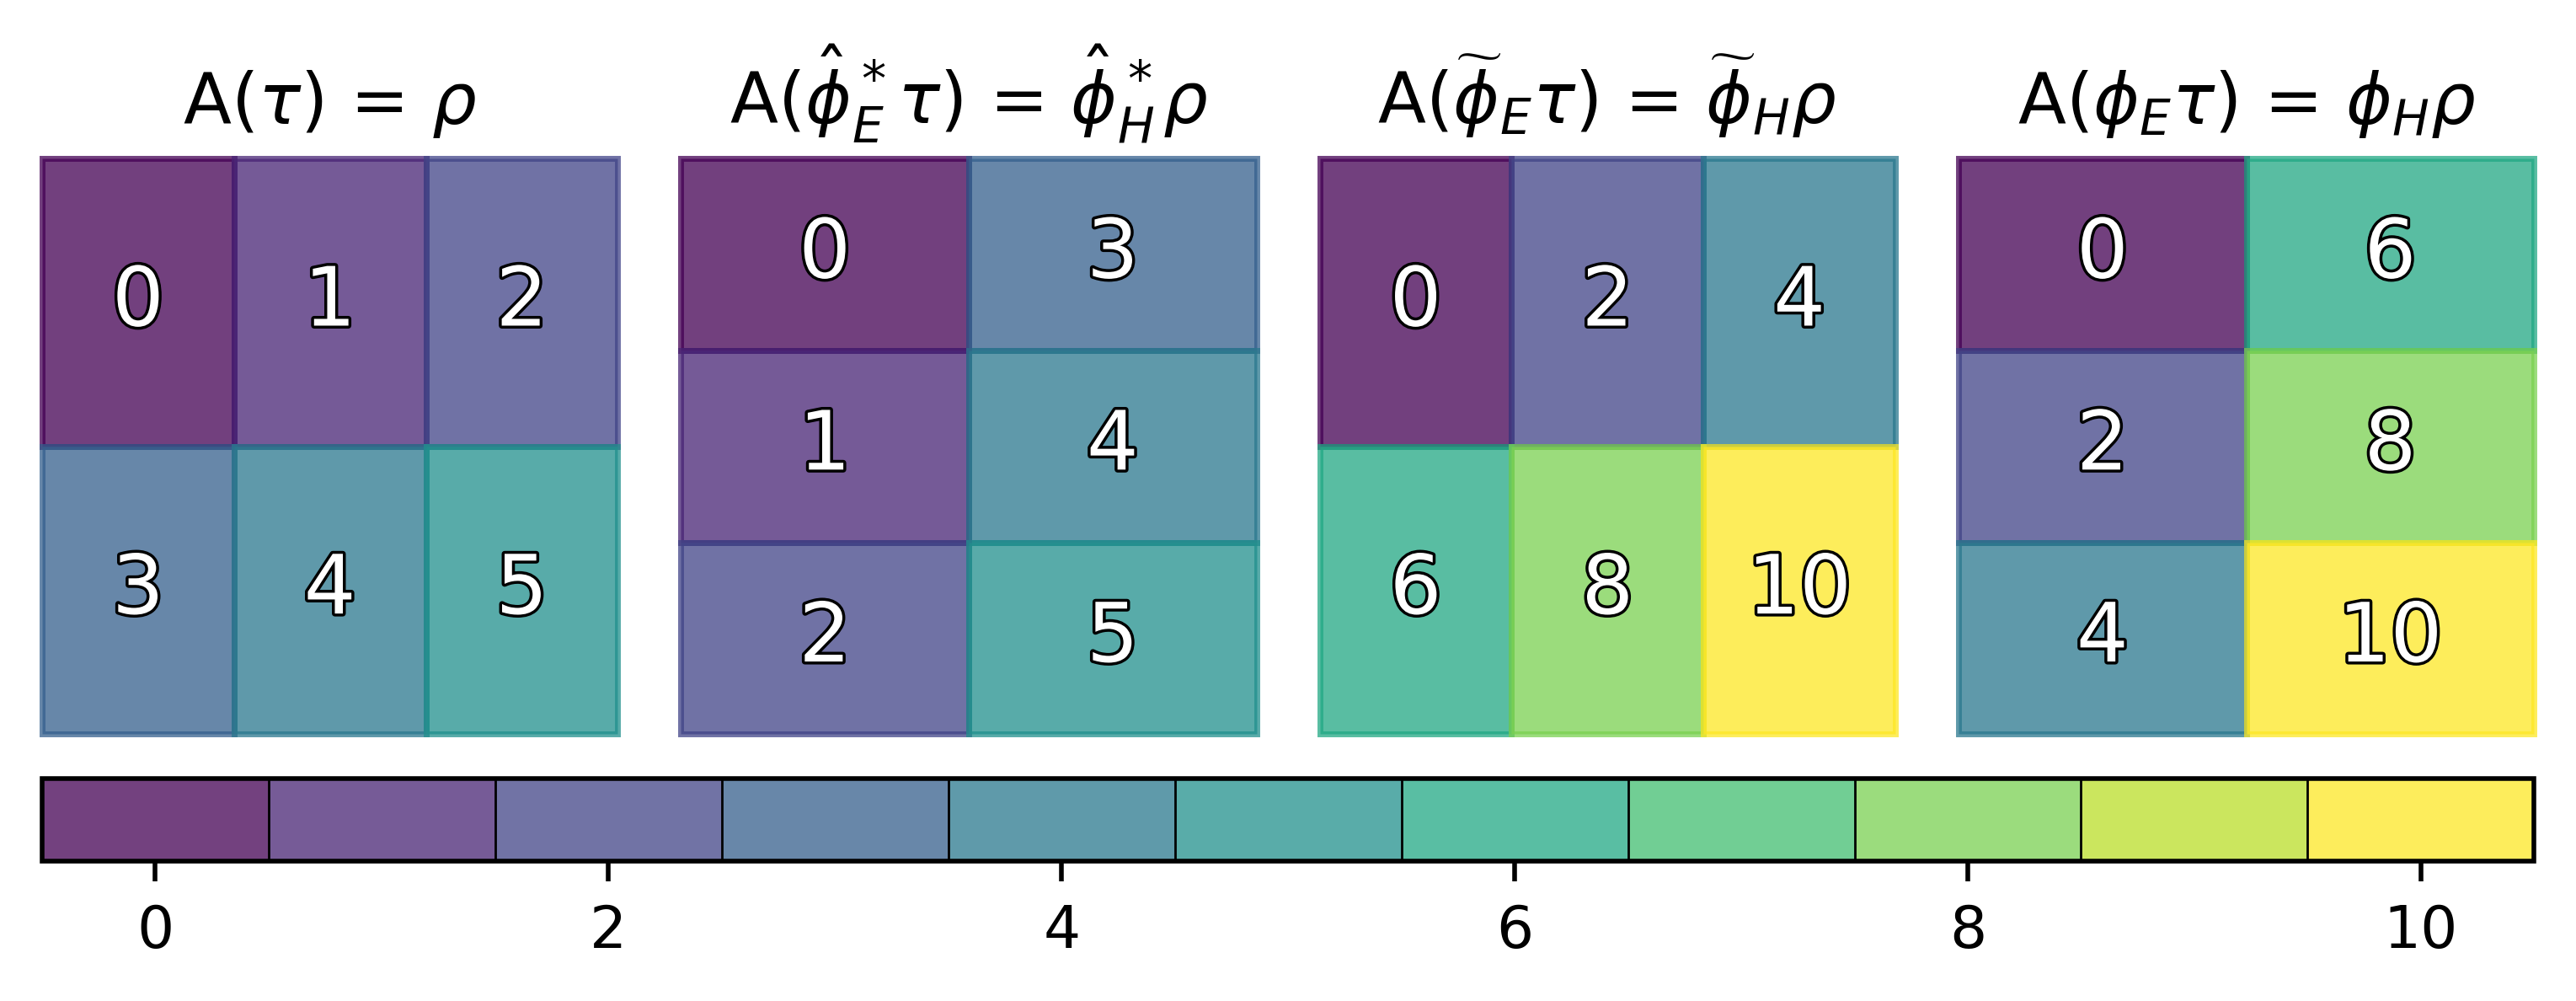
\includegraphics[width=1\columnwidth]{equivariance.png}
  \caption{This artist is equivariant because when the input data $\dsection$ is transposed, $\dfunch$, scaled $\dfunct$, and transposed and scaled $\dfunc$, the corresponding colored cells are transposed, scaled such that the color is moved two steps, and both transposed and scaled. 
  \label{fig:artist:equivariance}}
\end{figure}
For example, in \autoref{fig:artist:equivarance}, the measurable variable is color. This is a visual representation of the data shown in \autoref{fig:atct:phi}, and as such the equivariant transformations are an equivalent transposition and scaling of the colors. This visualization is equivariant with respect to base space transformations, as defined in \autoref{eq:atct:equivarance:verify:base}, because the color values at the new position at the old position $measure_\dbasepoint^{\prime} = \measure_{\dbasepoint}$. This visualization is also equivariant with respect to fiber wise transformations, as defined in \autoref{eq:atct:equivarance:verify:fiber}, because the colors are consistently scaled in the same was the data. For example, the values that have become 2 and 4 in the $\dfunctc$ and $\dfunc$ panels are colored the same as the original 2 and 4 values in the first panel. The equivariance in this visualization is composable, as shown in the colors being both transposed and scaled correctly in the $\dfunc$ panel.

\subsection{Composing Artists}\label{sec:artist:operators}
A common use of category theory in software engineering is the specification of modular components \cite{wielsManagementEvolvingSpecifications1998} such that we can build systems where the structure preserved by components is preserved in the composition of the components. This allows us to express that an artist that works on a dataset can be composed of artists that work on sub parts of that dataset. 
\begin{equation}
  \label{eq:artist:operator}
  \begin{tikzcd}[column sep=small]
      & \dfiberc^{a} \times_{\dfiberc^{c}} \dfiberc^{b} 
    \arrow[ld, "{\pi_{a\times b, a}}"', color=fiber] 
    \arrow[rd, "{\pi_{a\times b, b}}", color=fiber] & & 
    \dtotalc^{a} \oplus_{\dfiberc^{c}} \dtotalc^{b} 
    \arrow[ddd, "\pi"', color=total] \\
    \dfiberc^{a} 
    %\arrow[d, "\pi"', color=fiber] 
    \arrow[r, "{\pi_{a,c}}", color=fiber] 
    & \dfiberc^{c} & \dfiberc^{b} 
    %\arrow[d, "\pi", color=fiber] 
    \arrow[l, "{\pi_{b,c}}"', color=fiber] & \\
    \dbasec^{a} 
    \arrow[rd, "{\iota_{a, a+b}}"', color=base] 
    & \dbasec^{c} 
    \arrow[r, "{\iota_{c,b}}", color=base] 
    \arrow[l, "{\iota_{c,a}}"', color=base] 
    & \dbasec^{b} 
    \arrow[ld, "{\iota_{b, a+b}}", color=base] 
    &  \\
    & \dbasec^{a}\sqcup_{\dbasec^c}\dbasec^{b} & & 
    \dbasec^{a}\sqcup_{\dbasec^c}\dbasec^{b} 
    \arrow[uuu, "{\dsectionc^{a,b}}"', dashed, bend right, color=section]
  \end{tikzcd}
\end{equation}

\subsubsection{Addition: +}
\label{sec:artist:addition}
As illustrated in \autoref{eq:artist:operator}, data bundles can be combined by taking the disjoint  union of base spaces $\dbase^{a} \sqcup_{\dbase^c} \dbase^b$, where $\dbase^c$ is an overlap. When the fibers of each bundle are isomorphic $\dfiber^{a} \simeq \dfiber^{b}$, which we denote as $\dtotal$, this is analogous to adding more records to a dataset. We propose an addition operator that states that an artist that takes in a dataset can be constructed using artists that take as inputs subsets of the dataset

\begin{equation*}
  \label{eq:artist:addition}
  \vartistc_{a+b}(\cgamma{\dbasec^{a} \sqcup_{\dbase^c} \dbasec^b}{\dtotalc}) \coloneqq \vartistc_{a}(\cgamma{\dbasec^{a}}{\dtotalc}) + \vartistc_{b}(\cgamma{\dbasec^{b}}{\dtotalc}) 
\end{equation*}
As introduce in $\autoref{eq:artist:hom_transport}$, the artist returns a function $\gsection$. We assume that the output space is a trivial bundle, which means that $\gsectionc \in Hom(\gbase, \gfiber)$ because the output specification is the same at each point $\gbase$. This allows us to make use of the hom set adjoint property\note{find citation}\
\begin{equation*}
  Hom(\gbase^{a} + \gbasec^b, \gfiber) = Hom(\gbase^{a}, \gfiber) + Hom(\gbase^b, \gfiber)
\end{equation*} 
to define an artist constructed via addition as consisting of two distinct graphic sections
\begin{equation}
  \label{eq:artist:plus:output}
  \gsectionc(\gbasepointc) \coloneqq \begin{cases} \gsectionc^{a}(\gbasepointc) & \gbasepointc \in \vindexprec(\dbasec^{a}) \\
    \gsectionc^{b}(\gbasepointc) & \gbasepointc \in \vindexprec(\dbasec^{b})
  \end{cases}
\end{equation}
that are evaluated only if the input graphic point is an the graphic area that graphic section acts on. 

One way to verify that these artists are composable is to check that the return the same graphic on points in the intersection $\dbase^{c}$.  Given $\dbasepointc_{a} \in \dbasec_{c} \subset \dbasec_{a}$ and $\dbasepointc_{b} \in \dbasec_{c} \subset \dbasec_{b}$, if $\dbasepointc_{a} = \dbasepointc_{b}$ then

\begin{equation}
  \label{eq:artist:plus:verify}
  \begin{split}
  &\vartistc_{a+b}(\dsectionc^{a+b}(\dbasepointc_{a})) \\ 
  & = \vartistc_{a}(\dsectionc^{a}(\dbasepointc_{a})) = \vartistc_{b}(\dsectionc^{b}(\dbasepointc_{b}))
  \end{split}
\end{equation}
 for all $\dbasepointc_{a}, \dbasepointc_{b} \in \dbasec_{a}\bigsqcup\limits_{\dbasec_{c}} \dbasec_{b}$  
 
 \note{replace w/ a line plot w/markers}
 One example of an artist that is a sum of artists is a sphere drawer that draws different quadrants of a sphere $\vartist(\dsection) = \vartist_{1}(\dsection_{1}) + \vartist_{2}(\dsection_{2}) + \vartist_{3}(\dsection_{3}) \vartist_{4}(\dsection_{4})$. Given an input $\dbasepoint \in \dbase_4$ in the 4th quadrant, then the graphic section that would be executed is $\gsection_{4}$. If that point is also in the 3rd quadrant  $\dbasepoint \in \dbase_3$, then both artist outputs must return the same values $\gsection_{4}(\vindexprec(\dbasepoint)) = \gsection_{3}(\vindexprec(\dbasepoint))$. 


\subsubsection{Multiplication: $\times$}
\label{sec:artist:operator:multiplication}
As illustrated in \autoref{eq:artist:operator},  fibers that are a cartesian product of fiberspaces $\dfiber^{a} \times_{\dfiber^c} \dfiber^{b}$, where $\dfiber^c$ is any fiber that is present in both fibers, can be projected down into component fibers. In the trivial case where the base spaces are the same $\dbase^{a} = \dbase^{b} = \dbase$, this is equivalent to adding more fields to a dataset. 

\begin{equation*}
  \label{eq:artist:multiplication}
  \vartistc_{a \times b}(\cgamma{\dbase}{\dtotalc^{a\times b}}) \coloneqq \vartistc_{a}(\cgamma{\dbasec}{\dtotalc^{a}}) \times \vartistc_{b}(\cgamma{\dbasec}{\dtotalc^{b}}) 
\end{equation*}
which following from an adjoint property of homsets \note{find citation}
\begin{equation*}
  Hom(\gbase, \gfiber) \times Hom(\gbase, \gfiber) = Hom(\gbase, \gfiber\times \gfiber)
\end{equation*}
which means that the artists on the subsets of fibers can be defined 
\begin{equation}
  \gsectionc^{a \times b} = \{\gsectionc^{a}(\gbasepointc), \gsectionc^{b}(\gbasepointc)\}, \gbasepointc \in \vindexprec(\dbasec)
\end{equation} 
but that the signature of $\gsectionc^{a \times b}$ would be $\gbase \rightarrow \gfiber \times \gfiber$. Instead of having to special case the return type of artists that are compositions of multiple case, the hom adjoint \note{find cite} property
\begin{equation*}
  Hom(\gbase, \gfiber \times \gfiber) = Hom(\gbase+\gbase, \gfiber)
\end{equation*}
 means that multiplication can be considered as a special case of addition where $\dbase^{a} = \dbase^{b}$. While we discussed the trivial case in \autoref{sec:artist:addition}, there is no strict  requirement that $\dfiber^{a} = \dfiber^{b}$. 

One way to verify that these artists are composable is to check that they encode any shared fiber $\dfiber^{c}$ in the same way.

\begin{equation}
  \begin{split}
    &\extractmc(\vartistc_{a\times b}(\dsectionc^{a\times b}(\dbasepointc)))\restriction_{\dfiberc^{c}}\\ 
    &= 
    \extractmc(\vartistc_{a}(\dsectionc^{a}(\dbasepointc_{a})))\restriction_{\dfiberc^{c}} = \extractmc(\vartistc_{b}(\dsectionc^{b}(\dbasepointc_{b})))\restriction_{\dfiberc^{c}}
  \end{split}
\end{equation}

This expectation of using the same encoding for the same variable is a generalization of the concept of consistency checking of multiple view encodings discussed by Zening and Hullman \cite{hullmanKeeping2018}. This expectation can also be used to check that a multipart glyph is assembled correctly. For example, a box plot \cite{wickham40YearsBoxplots2011} typically consists of a rectangle, multiple lines, and scatter points; therefore a boxplot artist $\vartist_{boxplot} = \vartist_{rect} \times \vartist_{errors} \times \vartist_{line} \times \vartist_{points}$ must be constructed such that all the sub artists draw a graphic at or around the same x value. 

\begin{figure}[h!]
  \centering
  \includegraphics*[scale=.75]{qcom.png}
  \caption{The circle-line visual element can be constructed via $\gsection_{circle}$ + $\gsection_{line}$ functions that generate the circle and line elements respectively. This is equivalent to a $\gsection_{circle+line}$ function that takes as input the combined base space $\gbase_{circle} \sqcup \gbase_{line} = \gbase_{circle-line}$ and returns pixels in the circle-line element.  \label{fig:artist:operator}}
\end{figure}
There is no way to visually determine whether a visual element is the output of a single artist or a multiplied or added collection of artists. The circle-line visual element in \autoref{fig:artist:operator} can be a visual representation of a highlighted point intersecting with a line plot with the same fields. The same element can also be encoding some fields of a section in the circle and other fields of that section in the lines. \note{+*equive}
Although we have been discussing the trivial cases of adding observations or adding fields, this merging of artists in datasets can be generalized:
\begin{equation}
  \vartistc(\cgamma{\mathop{\sqcup}_{i} \dbasec^{i}}{\mathop{\oplus}_{i}\dtotalc^{i}}) \coloneqq \sum_{i}
  \vartistc_{i}(\cgamma{\dbasec^{i}}{\dtotalc^{i}}) 
\end{equation} 

As shown in \autoref{eq:artist:operator}, bundles over a union of base spaces can be joined as a product of the fibers. This allows us to consider all the data inputs in a complex visualization as a combined input, where some sections evaluate to null in fields for which there are no values for that point in the combined base space $\dbasepoint \in \mathop{\sqcup}_{i} \dbase^{i}$ The combined construction of the data is a method for expressing what each data input has in common with another data input-for example the data for labeling tick marks or legends- 
and therefore which commonalities need to be preserved in the artists that act on these inputs. 

\section{Construction}
\label{sec:construction}

We propose that one way of constructing artist functions is to separate generating a visualization, as shown in \autoref{fig:construction:flow}, is into an equivariant continuity preserving encoding stage $\vchannelc$ and a equivariant continuity preserving compositing stage $\vmarkc$. In the \textcolor{artist}{encoding} stage $\vchannelc$, a data bundle is treated as separable fields and each field is mapped to a measurable visual variable. In the encoding stage, the expected visual mappings $\equivb$ can be implemented inside the library. Factoring out the encoding stage leaves the \textcolor{artist}{compositing} stage $\vmarkc$ responsible for faithfully translating those measurable visual components into a visual element.  

\subsection{Measurable Visual Components}
\label{sec:construction:vtotal}
As shown in \autoref{fig:construction:flow}, we propose an intermediate visual fiber bundle 
\begin{equation}
  \vfiberc \hookrightarrow \vtotalc \xrightarrow{\pi} \dbasec
\end{equation}
where the space of possible visual encodings is the fiber space $\vfiber$. The space of visual sections which return visual encoding specifications is 
\begin{equation}
\cgamma{\opensetc}{\vtotalc\restriction_{\opensetc}} \coloneqq \big\{\vsectionc: \opensetc\rightarrow \vtotalc\restriction_{\opensetc} \; \bigm{\vert} \pi(\vsectionc(\dbasepointc)) = \dbasepointc\;for\, all\; \dbasepointc \in \opensetc \big\} 
\end{equation}
As shown in \autoref{eq:artist:inout:diagram},  measurable visual components are defined as having the same continuity as the data $\dbase$. This means that every data record $\dsection(\dbasepoint)$ has a corresponding visual section such that $\pi(\dsection(\dbasepoint)) = \pi(\vsection(\dbasepoint))$. 

Although the bundle $\vtotal$ is structurally equivalent to the bundle $\dtotal$, its existence allows for separating the data that is input into the artist $\dsection$ from the data internal to the artist $\vsection$. This allows a visualization library to define a visual bundle space $\vtotalc$ the holds the internal representation standard for measurable visual components. For example, a visualization library could define a visual color fiber as an RGBA tuple $\vfiber_{color} = \mathbb{R}^{3} \times [0,1]$. This would then set the expectation that arbitrary color encoding functions would need to return an RGBA tuple for the library to recognize the encoding as a color. 

\subsection{Map Between Graphics and Data}
In \autoref{sec:atct:sheaves}, the functors $\vindex, \vindexpull, \vindexpushc$ are introduced to describe the expected relationship between screen and data base spaces. In the construction of the artist, the functor $\vindex$ is defined such that the data base space \dbase\ is a deformation retraction\cite{nlab:deformation_retract} of the graphic space $\gbase$. This means that there is a continuous surjective mapping from every point $\dbasepoint\in\dbase$ to a point $\dbasepoint \in dbase$. To simplify matters, in this paper, we construct the graphic space as a constant multiple of the base space such that 
\begin{equation}
  \underbrace{\dbasec\times[0,1]^{n}}_{\gbasec} \textcolor{functor}{\xmapsto{\hspace{1em}\vindexc\hspace{1em}}} \dbasec
\end{equation}
where n is a thickening of the graphic base space $\gbase$ to account for the dimensionality of the output space
\begin{equation*}
  n = \begin{cases}
    dim(\gbase) - dim(\dbase) & dim(\dbase)<dim(\gbase)\\
  0 & otherwise
  \end{cases}
\end{equation*}
because the data dimensionality $\dbase$ may be too small for a graphic representation.

\begin{figure}[h!]

  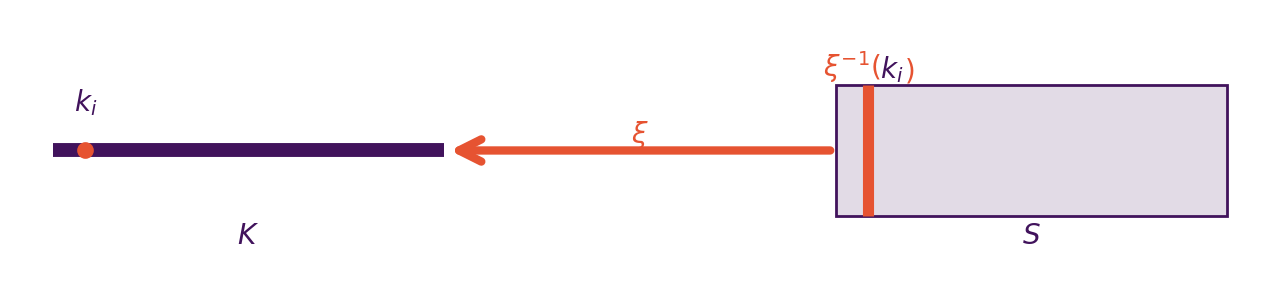
\includegraphics[width=1\columnwidth]{deform_retract.png}
  \caption{The graphic base space $\gbase$ is collapsable to the line $\dbase$ such that every band $(\dbasepoint_i, [0,1])$ on $\gbase$ maps to corresponding point $\dbasepoint_i \in \dbase$. The band $[0,1]$ determines the thickness of a rendered line for a given point $\dbasepoint_{i}$ by specifying how pixels corresponding to that point are colored. \label{fig:construction:xi}}
\end{figure}

For example, as shown in \autoref{fig:construction:xi}, a line is 1D but is a 2D glyph on a screen; therefore the graphic space $\gbase$ is constructed by multiplying the base space $\dbase$ with an interval $[0,1]$. Because $\gbase$ is collapsible into $\dbase$, every band $(\dbasepoint_i, [0,1])$ corresponds to a point in the base space $\dbasepoint_i \in \dbase$. The first coordinate $\alpha=\dbasepoint_i$ provides a lookup to retrieve the associated visual variables. The second coordinate, which is a point in the interval $\beta=[0,1]$. Together they are a point $\gbasepoint=(\alpha,\beta) \in gbase$ in the graphic base space. This point $\gbasepoint$ is the input into the graphic section $\gsection(\gbasepoint)$ that is used to determine which pixels are colored, which in turn determines the thickness, texture, and color of the line. 


\subsection{Component Encoders}
\label{sec:construction:nu}
As introduced in \autoref{fig:construction:flow}, the encoding function $\vchannel$ is a map from data sections to graphic sections
\begin{equation}
\nu: \cgamma{\dbasec}{\dtotalc} \rightarrow \cgamma{\dbasec}{\vtotalc}
\end{equation}
such that the sections project to the same point on the base space $\pi(\dtotal) = \pi(\vchannel(\dtotal))$. A consequence of this property is that $\vchannelc$ can be constructed as a pointwise transformation such that  
\begin{equation}
  \label{eq:constrution:nu}
  \vchannelc: \dfiberc_{\dbasepointc} \rightarrow \vfiberc_{\dbasepoint}
\end{equation}
which means that means that a point in a single data fiber $\delement \in \dfiber_{\dbasepointc}$ can be mapped into a corresponding point in a visual fiber $\velement \in \vfiber_{\dbasepointc}$. This means that an encoding function $\vchannel$ can convert a single record and may not need the whole dataset. 

The difference between $\dtotal$ and $\vtotal$ are semantic rather than structural; they are both maps from the topological space \dbase\ to sets of functions that return records of values. This means any $\vtotal$ can be redefined as $\dtotal$, 
\begin{equation}
  \label{eq:construction:nu:fabrication}
  \begin{tikzcd}[col sep=Huge]
    \dfiberc_{\dbasepointc} 
    \arrow[rr, "\vchannelc", color=artist] 
    \arrow[rrrr, "\vchannelc^{\prime\prime}", dashed, bend right, color=artist] &  & 
    \vfiberc_{\dbasepointc}\coloneqq{\dfiberc_{\dbasepointc}^{\prime}} 
    \arrow[rr, "\vchannelc^{\prime}", color=artist] &  & 
    \vfiberc^{\prime}_{\dbasepointc}
  \end{tikzcd}
\end{equation}
which means that, as shown in \autoref{eq:construction:nu:fabrication}, any collection of $\vchannel$ functions can be composed such that they are equivalent to a $\vchannel$ that directly converts the input to the output. As with artists, $\vchannel$ are maps of sections such that the composition operators defined in \autoref{sec:artist:composition} can also act on transformers $\vchannel$, meaning that encoders can be added $\vchannel_{a+b} = \vchannel_{a} + \vchannel_{b}$ and multiplied d $\vchannel_{a\times b} = \vchannel_{a}  \vchannel_{b}$.  Encoders designed to satisfy these composability constraints provide for a rich set of building blocks for implementing complex encoders.

\subsubsection{Encoder Verification}
\label{sec:construction:nu:verification}
A  motivation for constructing an artist with an encoder stage $\vchannel$ is so that the conversion from data to measurable component can be tested separately from the assembly of components into a glyph. 
\begin{equation}
  \label{eq:construction:nu:validate}
  \begin{tikzcd}[column sep=4em]
    {\dfiberc_{\dbasepointc}^{a}} \times {\dfiberc_{\dbasepointc}^{b}} 
    \arrow[d, "\pi_a"', color=fiber] 
    \arrow[r, "\vchannelc_{ab}", color=artist] 
    \arrow[rr, "\equivc_{ab}", bend left, color=monoid]  & 
    {\vfiberc_{\dbasepointc}^{a}} \times {\vfiberc_{\dbasepointc}^{b}} 
    \arrow[d, "\pi_a", color=fiber] & 
    \measurec_{\dbasepointc}^{ab} 
    \arrow[d, "\measurec\restriction_a", color=set] \\
    \dfiberc_{\dbasepointc}^a 
    \arrow[r, "\vchannelc_{a}", dashed, color=artist] & 
    \vfiberc_{\dbasepointc}^a 
    \arrow[r, "\simeq", dotted]  & 
    \measurec_{\dbasepointc}^a   \\
    {\dfiberc_{\dbasepointc}^{a}} \times {\dfiberc_{\dbasepointc}^{c}} 
    \arrow[u, "\pi_a", color=fiber] 
    \arrow[r, "\vchannelc_{ac}", color=artist] 
    \arrow[rr, "\equivc_{ac}", bend right, color=monoid] & 
    {\vfiberc_{\dbasepointc}^{a}} \times {\vfiberc_{\dbasepointc}^{c}} 
    \arrow[u, "\pi_a"', color=fiber] & 
    \measurec_{\dbasepointc}^{ac} 
    \arrow[u, "\measurec\restriction_a"', color=set]            
    \end{tikzcd}
\end{equation}
As shown in \autoref{eq:construction:nu:validate}, an encoder is considered valid if there is an ismorphism between the actual outputted visual component and the expected measurable component encoding. An encoder is consistent if it encodes the same field in the same way even if coming from different data sources. 

An encoding function $\vchannelc$ is equivariant if the change in data, as defined in \autoref{sec:atct:sheaves:measurments}, and change in visual components are equivariant. Since $\dtotal$ and $\vtotal$ are over the same base space and are pointwise, the base space change $\dfunch_{\dtotal}$ applies to both sides of the equation 
\begin{equation}
  \vchannelc(\dsectionc_{\dtotalc}(\dfunchc_{\dbasec}(\dbasepointc^{\prime}))) = \vsectionc(\dfunchc_{\dbasec}(\dbasepointc^{\prime}))
\end{equation}
and therefore there should not be a change in encoding. On the other hand, a change in the data values $\dfunct_{\dtotal}$ must have an equivalent change in visual components
\begin{equation}
  \dfunctc_{\vtotalc} \vchannelc(\dsectionc(\dbasepoint)) = \vchannelc(\dfunctc_{\dtotalc}(\dsectionc(\dbasepointc)))
\end{equation}
The change in visual components $\dfunct_{\vtotal}$ is dependent both on $\dfunct_{\dtotal}$ and the choice of visual encoding. As mentioned in \autoref{sec:related-work:equivariance}, this is why Bertin and many others since have advocated choosing an encoding that has a structure that matches the data structure\cite{bertinSemiologyGraphicsDiagrams2011a}. For example choosing a quantative colormap to encode quantative data if the $\dfunctc$ operation is scaling, as in \autoref{fig:artist:equivariance}.


\subsection{Graphic Compositor}
As shown in \autoref{fig:construction:flow}, the compositor function $\vmarkc$ transforms the measurable components into properties of a visual element. The compositing function $\vmarkc$ transforms the sections of visual elements $\vsectionc$ into sections of graphics $\gsectionc$.
\begin{equation}
  \vmarkc: \cgamma{\dbasec}{\vtotalc} \rightarrow \cgamma{\gbasec}{\gtotalc}
\end{equation}
The compositing function is map from sheaves over $\dbase$ to sheaves over $\gbase$. This is because, as described in \autoref{fig:construction:xi}, the graphic section must be evaluated on all points in the graphic space to generate the visual element corresponding to a data record at a single point $\vartist(\dsection(\dbasepoint)) = \gsection(\vindexpre(\dbasepoint))$. 

Since encoder functions are infinitely composable, as described in \autoref{eq:construction:nu:fabrication}, a new compositor function $\vmarkc$ can be constructed by precomposing $\vchannelc$ functions with the existing $\vmarkc$.

\begin{equation}
  \label{eq:construction:q:fabrication}
  \begin{tikzcd}
      \cgamma{\dbasec}{\vtotalc} 
      \arrow[rr, "\vchannel", color=artist] 
      \arrow[rrrr, "\vmarkc^{\prime}", bend right, color=artist, dashed] &  & \cgamma{\dbasec}{\vtotalc^{\prime}} 
      \arrow[rr, "\vmarkc", color=artist] &  & \cgamma{\gbasec}{\gtotalc}
      \end{tikzcd} 
\end{equation}
The composition in \autoref{eq:construction:q:fabrication} means that different measurable components can yield the same visual elements. The composition operators defined in \autoref{sec:artist:composition} can also act on compositors $\vmark$ such that $\vmark_{a+b} = \vmark_{a} + \vmark_{b}$ and multiplied d $\vmark_{a\times b} = \vmark_{a}  \vmark_{b}$.  


\begin{figure}[h!]
  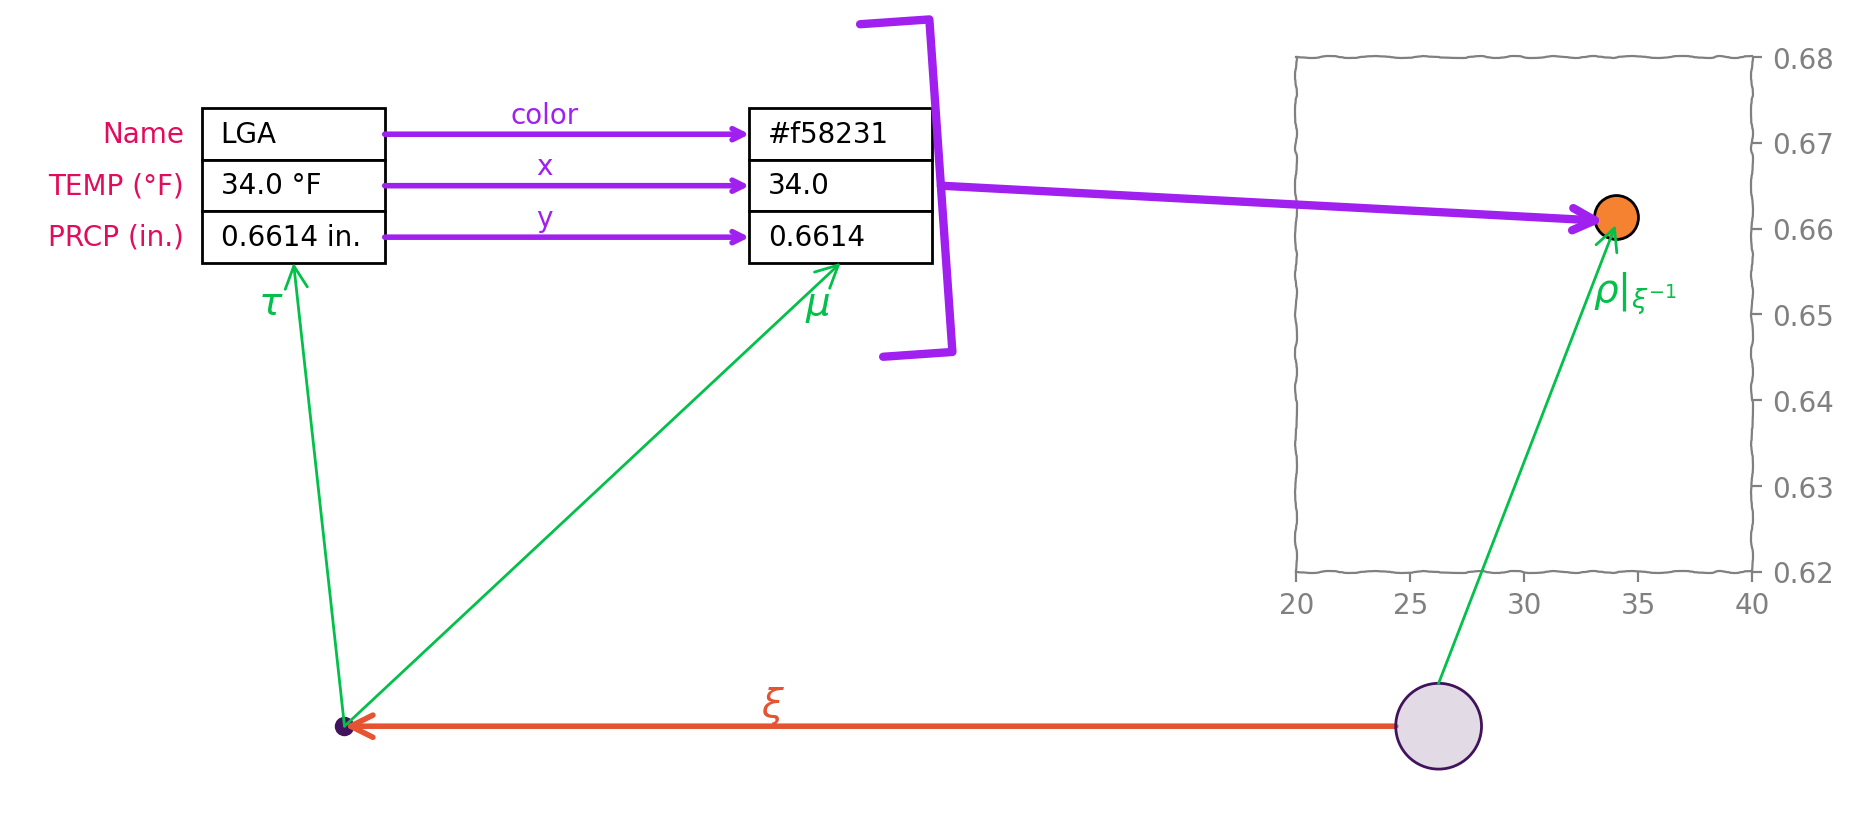
\includegraphics[width=1\columnwidth]{full_scatter.png}
  \caption{This simple $\vmarkc$ assembles a circular visual element that is the color specified in $\vsection(\dbasepoint)$ and is at the intersection specified in $\vsection(\dbasepoint)$ \label{fig:construction:q}}
\end{figure}
As shown in \autoref{fig:construction:q}, a set of  $\vchannel$ functions individually convert the values in the data record to visual components. Then the $\vmark$ function combines these visual encodings to produce a graphic section \gsection. When this section is evaluated on the graphic space associated with the data $\gsection(\vindexpre(\dbasepoint))$, it produces a blue circular marker at the intersection of the x and y positions listed in \vsection. The composition rule in \autoref{eq:construction:q:fabrication} means that developers can implement $\vmark$ as drawing circles or can implement a $\vmark$ that draws arbitrary shapes, and then provide different $\vchannel$ adapters, such as one that specifies that the shape is a circle. 

\subsubsection{Compositor Verification}
\label{sec:construction:q:verification}
An advantage of factoring out encoding and verification, as discussed in \autoref{sec:construction:nu:verification}, is that the responsibility of the compositor can be scoped to translating measurable components into visual elements. 
\begin{equation}
  \label{eq:construction:q:validate}
  \begin{tikzcd}[row sep=huge]
    \cgamma{\dbasec}{\vtotalc^{a}\times \vtotalc^{b}}  
    \arrow[rr, "\vmarkc_{ab}", color=artist] 
    \arrow[d, "\pi_a"', color=total] &  &  \imartistsub{ab}{\gbasec}{\gtotalc} 
    \arrow[d, "\measurec\restriction_a \circ \extractmc_{ab}", color=monoid]  \\
   \cgamma{\dbasec}{\vtotalc^{a}} 
   \arrow[rr, "\simeq", dotted] &  & 
   {\textcolor{set}{Hom}(\dbasec, \measurec^{a})}  \\
    \cgamma{\dbasec}{\vtotalc^{a}\times \vtotalc^{c}}  
    \arrow[rr, "\vmarkc_{ac}", color=artist] 
    \arrow[u, "\pi_a", color=total]  &  &  \imartistsub{ac}{\gbasec}{\gtotalc} 
    \arrow[u, "\measurec\restriction_a \circ \extractmc_{ac}"', color=monoid]
   \end{tikzcd}
\end{equation}
As illustrated in \autoref{eq:construction:q:validate}, a compositor is valid if there is an isomorphism between the actual outputted measured visual component and the expected measurable component that is the input. One way of verifying that a compositor is consistent is by verifying that it passes through one encoding even while changing others. For example, when $\vmark_{ab}=\vmark_{ac}$ then the output should differ in the same measurable components as $\vsectionc_{ab}$ and $\vsection_{ac}$. 

A compositor function \vmark\ is equivariant if the renderer output changes in a way equivariant to the data transformation defined in \autoref{sec:atct:sheaves:measurments}. This means that a change in base space $\dfunch_{\dtotalc}$ should have an equivalent change in visual element base space. This means that there should be no change in visual measurement
\begin{equation}
  \label{eq:construction:q:verification:base}
  \vsectionc(\dfunchc_{\dbasec}(\dbasepointc^{\prime})) = \extractmc(\vmarkc(\vsectionc)(\dfunch_{\dbasec}(\vindexprec^{\dbasepointc}))) = \measurec_{\dbasepointc}
\end{equation}
As discussed in \autoref{fig:artist:equivariance}, the change in base space may induce a change in locations of measurements relative to each other in the output; this can be verified via checking that all the measurements have not changed relative to the original positions $\measurec_{\dbasepoint} = \measurec_{\dbasepointc^{\prime}}$ and through separate measurable variables that encode holistic data properties, such as orientation or origin. 

The compositor function is also expected to be equivariant with respect to changes in data and measurable components
\begin{equation}
  \label{eq:construnction:q:verify:base}
  \dfunctc_{\vtotalc}(\vsectionc(\dbasepointc)) = \dfunctc_{\measurec}(\vmarkc(\vsectionc(\dbasepointc)))  
\end{equation}
which means that any change to a measurable component input must have a measurably equivalent change in the output. As illustrated in \autoref{fig:artist:equivariance}, the compositor $\vmarkc$ is expected to assemble the measurable components such that base space changes, for example transposition, are reflected in the output; faithfully pass through equivariant measurable components, such as scaled colors; and ensure that both types of transformations, here scaling and transposition, are present in the final glyph.  

\subsection{Implementing the Artist: $\vartistc=\vmarkc\circ\vchannelc$}

As shown in \autoref{eq:atct:sheaves:homset}, if a sheaf is equipped with transport functors, then the functions between sheaves over one space are isomorphic to functions between sheave over the other space. This property, allows us to specify the transformation from data to graphic space in data or graphic space or a combination, as listed in \autoref{eq:artist:hom_transport}, such that the following diagram commutes:
\begin{equation}
  \label{eq:construction:artist:path}
\begin{tikzcd}[row sep=2.5em, column sep=1.5em]
  \cgamma{\dbasec}{\dtotalc} 
  \arrow[rr, "\vchannelc^{\dbasec}", color=artist] 
  \arrow[rrrr, "\vartistc^{\dbasec}", bend left, color=artist] 
  \arrow[dd, "\vindexpullc"', color=functor] 
  \arrow[rrrrdd, "\vartistc", color=artist, pos=.2] &  & 
  \cgamma{\dbasec}{\vtotalc} 
  \arrow[rrdd, "\vmarkc", color=artist] 
  \arrow[rr, "\vmarkc^{\dbasec}", color=artist] 
  \arrow[dd, "\vindexpullc", color=functor, pos=.2] &  & \imartist{\dbasec}{\vindexpushc\gtotalc}  \\
   & & & & \\
  \cgamma{\gbasec}{\vindexpullc\dtotalc} 
  \arrow[rr, "\vchannelc^{\gbasec}", color=artist] 
  \arrow[rrrr, "\vartistc^{\gbasec}", bend right, color=artist] & & 
  \cgamma{\gbasec}{\vindexpullc\vtotalc} 
  \arrow[rr, "\vmarkc^{\gbasec}", color=artist] &  & 
  \imartist{\gbasec}{\gtotalc} 
  \arrow[uu, "\vindexpushc"', color=functor]
\end{tikzcd}  
\end{equation}
The diagram in \autoref{eq:construction:artist:path} illustrates how a developer can connect transformations over data space, denoted with a subset $\dbase$, with transformations over graphic space $\gbase$, using $\vindexpushc$ and $\vindexpullc$ adaptors. This allows developers to for example connect transformers that transform data on a line to a color in dataspace, but build a line compositing function that dynamically resamples what is on screen in graphic space.
\begin{figure}
  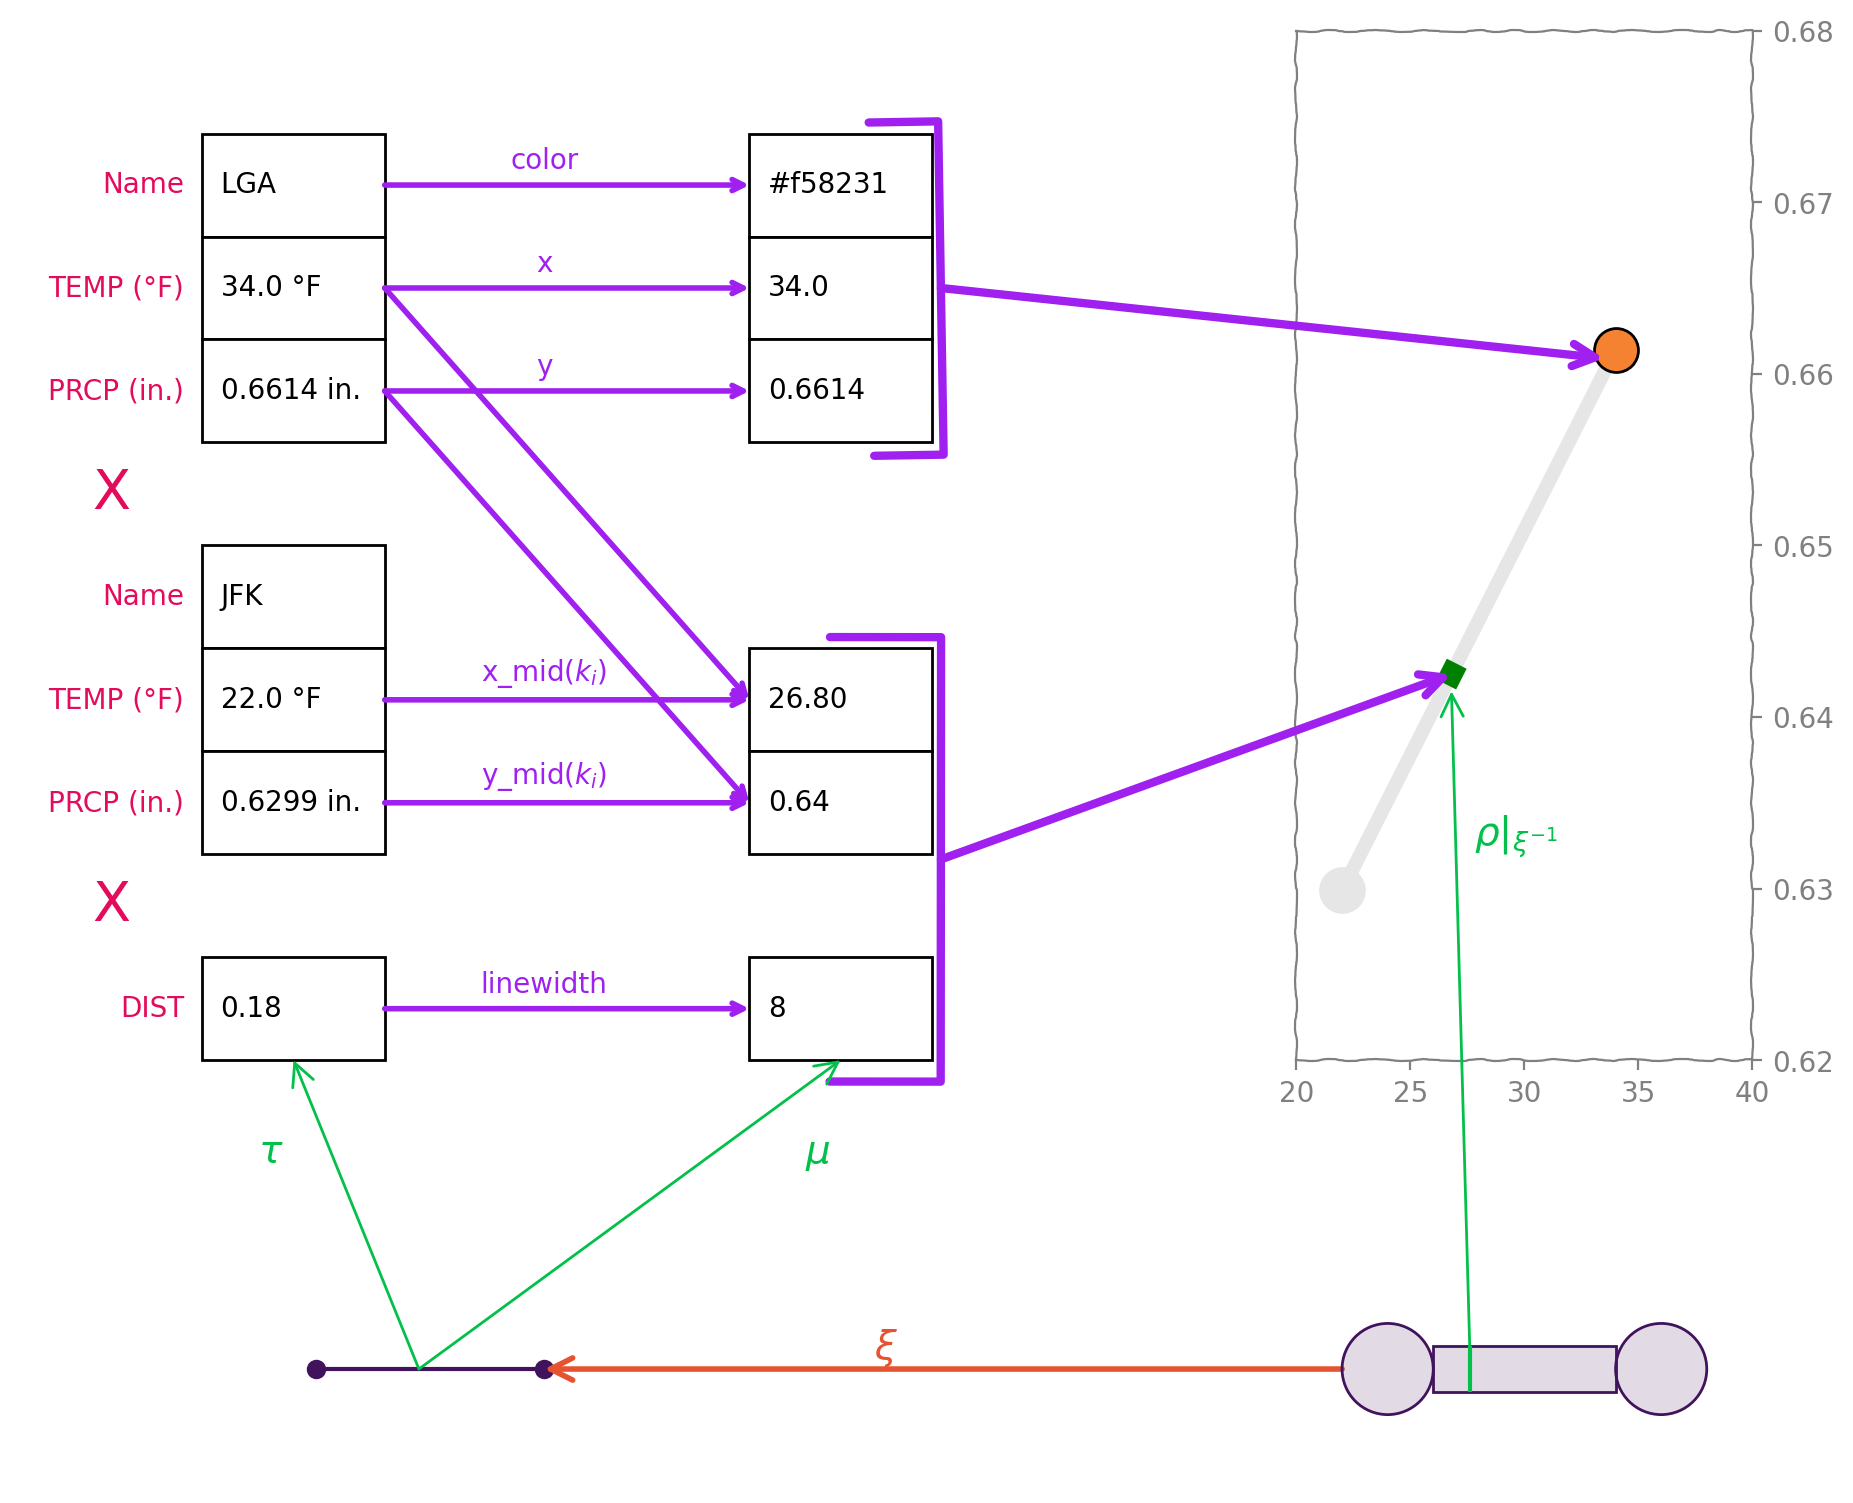
\includegraphics[width=1\columnwidth]{full_line.png}
  \caption{\label{fig:construction:artist:combo}}
\end{figure}

\section{Discussion: Feasibility of Math as Design Spec}
\label{sec:discussion}
The framework specified in \autoref{sec:artist} and \autoref{sec:construction} describes how to build structure preserving visualization components, but it is left to the library developer to follow these guidelines when building and reusing components. In this section, we introduce a toy example of building an artist out of the components introduced in \autoref{sec:construction} to illustrate how components that adhere to these specifications are maintainable, extendible, scalable, and support concurrency. 

\begin{figure}[h!]
  \centering
  \subfloat[]{
    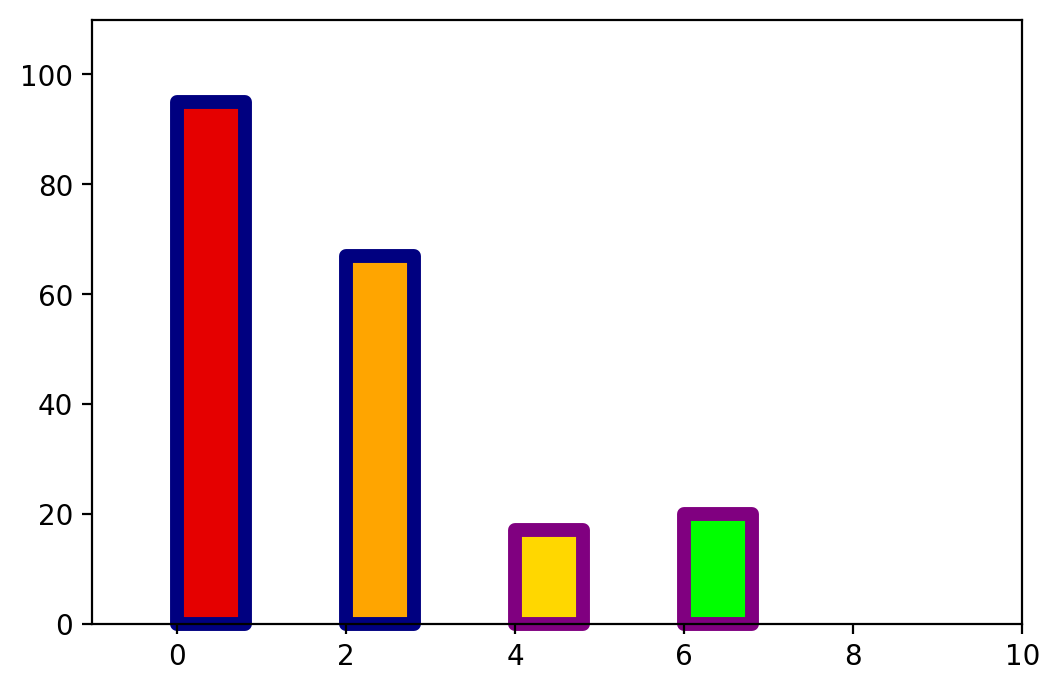
\includegraphics[width=.45\columnwidth]{bar.png}
  \label{fig:discussion:vbar}}
  \subfloat[]{
    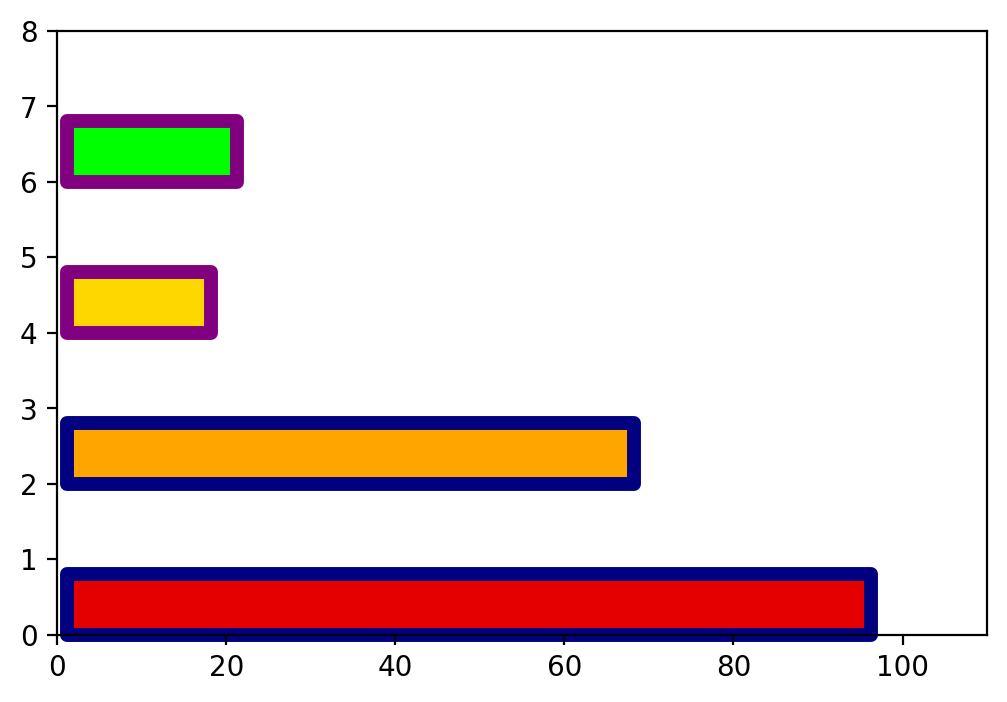
\includegraphics[width=.45\columnwidth]{barh.png}
  \label{fig:discussion:hbar}
  }
  \label{fig:discussion:bar}
\end{figure}

Specially, we introduce artists for building the graphical elements shown in \autoref{fig:discussion:bar} because it is a visualization type that allows us to demonstrate composability and multivariate data encoding. We build our visualization components by extending the Python visualization library Matplotlib's artist\footnote{Matplotlib artists are our artist's namesake}\cite{hunterMatplotlib2DGraphics2007,hunterArchitectureOpenSource} to show that components using this model can be incorporated into existing visualization libraries iteratively. While the architecture specified in \autoref{sec:construction} can be implemented fully functionally, we make use of objects to keep track of parameters passed into artists. In this toy example, the small composable components allow for more easily verifying that each component does its transformation correctly before assembling them into larger systems.  

\subsection{Bundle Inspired Data Containers}
\begin{table}[h!]
  \centering
\begin{tabular}{|lcl|}
  \hline \\
   fruit &  calories &  juice \\
  \hline\\
    apple &        95 &   True \\ 
   orange &        67 &   True \\ 
  lemon &        17 &  False \\ 
      lime &        20 &  False \\
  \hline
\end{tabular}
\label{tab:discussion:data}
\end{table}
We construct a toy dataset with a discrete $\dbase$ of 4 points and a fiber space of $\dfiber=\{apple,\, orange,\, lemon\}\times \mathbb{Z}^{+} \times \{\texttt{True}, \texttt{False}\}$. We thinly wrap \autoref{tab:discussion:data} in an object so that the common data interface function is that $\tau = \ttexttt{DataContainerObject.query}$. 
\begin{minted}{python}
  class FruitFrameWrapper:
    def query(self, data_bounds, sampling_rate):
      # local sections are a list of
      # {field: local_batch_of_values}
      return local_sections
\end{minted}

This interface provides a uniform way of accessing subsets of the data, which are local sections. The motivation for a common data interface is that it would allow the artist to talk to different common python data containers, such as numpy\cite{harris2020array}, pandas\cite{jeff_reback_2020_3715232}, xarray \cite{hoyer2017xarray}, and networkx\cite{HagbergExploringNetwork2008}. Currently, data stored in these containers must be unpacked and converted into arrays and matrices in ways that either destroy or recreate the structure encoded in the container. For example a pandas data frame must be unpacked into its columns before it is sent into most artists and continuity is implicit in the columns being the same length rather than a tracked base space $\dbase$. Because it is more efficient to work with the data in column order, we often treat the data as a collection of single fiber bundles. This is equivalent to the total bundle, as shown in \autoref{eq:artist:operator}. 

\subsection{Component Encoders}
To encode the values in the dataset, we enforce equivariance by writing $\vchannel$ encoders that match the structure of the fields in the dataset. For example, the fruit column is a nominal measurement scale. Therefore we implement a position encoder that respects permutation $\dfunch$ transformations. The most simple form of this $\vchannel$ is a python dictionary that returns an integer position, because Matplotlib's internal parameter space expects a numerical position type. 
\begin{minted}{python}
  def position_encoder(val):
    return {'apple': 0, 'orange': 2, 'lemon': 4, 'lime': 6}[val]
\end{minted}
As mentioned in \autoref{eq:construction:nu:fabrication}, the encoders can be composed up. For example, the compositor $\vchannel$ may need the position to be converted to screen coordinates. Here the screen coordinate $\vchannel$ is a method of a Matplotlib axes object; a Matplotlib axes is akin to a container artist that holds all information about the sub artists plotted within it. 
\begin{minted}{python}
def composite_x_transform(ax, nu):
    return lambda x: ax.transData.transform(
            (position_encoder(x), 0))[0]
\end{minted}
This encoder returns a function that is \texttt{transData.transform} $\vchannel_{transData}$ composed with the position encoder $\vchannel_{position}$ and takes as input a record to be encoded. As with the position encoder, the transData encoder respects permutation transforms because it returns reals; therefore the composite encoder respects permutation transforms. In this model, developers implement $\vchannel$ encoders that are explicit about which $\dfunc_{\vtotal}$ they support. Writing semantically correct encoders is also the responsibility of the developer and is not addressed in the model. For example \mintinline{python}{fruit_encoder = lamda x: {'apple': green, 'orange':'yellow', 'lemon':'red', 'lime':'orange'}} is a valid color encoding with respect to permutation, but none of those colors are intuitive to the data. It is therefore left to the user, or domain specific library developer, to choose $\vchannel$ encoders that are appropriate for their data.

\subsection{Graphic Compositors}
After converting each record into an intermediate visual component $\vsection$, the set of visual records is passed into $\vmarkc$. Here the $\vmarkc$ includes one last encoder, as illustrated in \autoref{eq:construction:q:fabrication}, that assembles the independent visual components into a rectangle. This $\vchannel$ is inside the $\vmarkc$ to hide that library preferred format from the user. It is called \texttt{qhat} to indicate that this is the $\vartist^{\dbase}$ path in \autoref{eq:construction:artist:path}.  This means that the parameters are constructed in data space $\dbase$ and this function returns a pushed forward $\vindexpush\gsection$. 

\begin{minted}{python}
   def qhat(position, width, length, floor, facecolor, edgecolor, linewidth, linestyle): 
        box = box_nu(position, width, length, floor)
        def fake_draw(render, transform=mtransforms.IdentityTransform()):
            for (bx, fc, ec, lw, ls) in zip(box, facecolor, edgecolor, linewidth, linestyle):
                gc = render.new_gc()
                gc.set_foreground((ec.r, ec.g, ec.b, ec.a))
                gc.set_dashes(*ls)
                gc.set_linewidth(lw)
                render.draw_path(gc=gc, path=bx, transform=transform, rgbFace=(fc.r, fc.g, fc.b, fc.a))
        return fake_draw
\end{minted}
The function \texttt{fake\_draw} is the analog of $\vindexpush\gsection$. This function builds the rendering spec through the renderer API, and this curried function is returned. The transform here is required for the code to run, but is set to identity meaning that this function directly uses the output of the position encoders. The curried $\texttt{fake\_draw} \approx \vindexpush \gsection$ is evaluated using a renderer object. In our model, as shown in \autoref{eq:artist:inout:diagram}, the renderer is supposed to take $\gsection$ as input such that $renderer(\gsection) = visualization$, but here that would require an out of scope patching of the Matplotlib render objects. 

One of the advantages of this model is that it allows for succinctly expressing the difference between two very similar visualizations, such as \autoref{fig:discussion:vbar} and \autoref{fig:discussion:hbar}. In this model, the horizontal bar is implemented as a composition of a $\vchannel$ that renames fields in $\vsection_{barh}$ and the $\vmark$ implementation for the horizontal bar.
\begin{minted}{python}
def qhat(length, width, position, floor, facecolor, edgecolor, linewidth, linestyle):
  return Bar.qhat(**BarH.bar_nu(length, width, position, floor, facecolor, edgecolor, linewidth, linestyle))
\end{minted}
This composition is equivalent to $\vmark_{barh} = \vmark_{bar} \circ \vchannel_{vtoh}$, which is an example of \autoref{eq:construction:q:fabrication}. These functions can be further added together, as described in \autoref{sec:artist:operators} to build more complex visualizations. 

\subsection{Integrating Components into an Existing Library}
The $\vchannel$ and $\vmark$ are wrapped in a container object that stores the $\vartist = \vmark \circ \vchannel$ composition and a method for computing the $\vsectionc$.
\begin{minted}{python}
  class Bar: 
    def compose_with_nu(self, pfield, ffield, 
          nu, nu_inv:):
        # returns a new copy of the Bar artist 
        # with the additional nu that converts 
        # from a data (F) field value to a 
        # visual (P) field value
        return new

    def nu(self, tau_local): #draw
       # uses the stored nus to convert data
       # stored nus have F->P field info
      return mus
    
    @staticmethod
    def qhat(position, width, length, floor, facecolor, edgecolor, linewidth, linestyle):
       
        return fake_draw
\end{minted}

This artist is then passed along to a shim artist that makes it compatible with existing Matplotlib objects
\begin{minted}{python}
class GenericArtist(martist.Artist):
    def __init__(self, artist:TopologicalArtist):
        super().__init__()
        self.artist = artist
        
    def compose_with_tau(self, section):
        self.section = section

    def draw(self, renderer, bounds, rate):
        for tau_local in self.section.query(bounds, rate): 
            mu = self.artist.nu(tau_local)
            rho = self.artist.qhat(**mu)
            output = rho(renderer)
\end{minted}
As shown in the \texttt{draw} method, generating a graphic section $\gsection$ is implemented as the composition of $\texttt{qhat} \approx \vmark$ and $\texttt{nu} \approx \vchannel$ applied to a local section of the sheaf $\textttt{self.section.query} \approx \desection^{i}$ such  $\texttt{draw} \approx \vmarkc\circ\vchannelc\circ\dsectionc  = \vartistc\circ \dsectionc$. The $\vchannel$ and $\vmark$ functions shown here are written such that they can generate a visual element given a local section $\dsection\restriction_{\dbase^{i}}$ which can be as little or large as needed. This flexibility is a prerequisite for building scalable and streaming visualizations that may not have access to all the data.  

The \texttt{GenericArtist} is a a standard Matplotlib object; therefore it can be hooked into the Matplotlib draw tree to produce the vertical bar chart in \autoref{fig:discussion:vbar}. Using the Matplotlib artist framework means this new artist can be composed with existing artists, such as the ones that draw the axes and ticks. 



The example in this section is intentionally trivial to illustrate that the math to code translation is fairly straightforward and results in fairly self contained composable functions. Further research could investigate building new systems using this model, specifically libraries for visualizing domain specific structured data and domain specific artists. More research could also explore applying this model to visualizing high dimensional data, particularly building artists that take as input distributed data and artists that are concurrent. Developing complex systems could also be an avenue to codify how interactive techniques are expressed in this framework.


\section{Conclusion}
The toy example presented in \autoref{sec:discussion} demonstrates that it is relatively straightforward to build working visualization library components using the construction described in \autoref{sec:construction}. Since these components are defined with single record inputs, the can be implemented such that they are concurrent. The cost of building a new function using these components is sometimes as small as renaming fields, meaning the new feature is relatively easy to maintain. These new components are also a lower maintenance burden because, by definition, they are designed in conjunction with tests that verify that they are equivariant.  
These new components are also compatible with the existing library architecture, allowing for a slow iterative transition to components built using this framework. 
The framework introduced in this paper is a marriage of the ways the graphic and data visualization communities approach visualization. The graphic community prioritizes \note{?} how input is translated to output, which is encapsulated in the artist $\vartist$. The data visualization community prioritizes the manner in which that input is encoded, which is encapsulated in the separation of stages $\vmark \circ \vchannel$. Formalizing that both views are equivalent $\vartist=\vmark \circ \vchannel$ gives library developers the flexibility to build visualization components in the manner that makes more sense for the domain without having to sacrifice the equivariance of the translation. 

\appendices



% use section* for acknowledgment
\ifCLASSOPTIONcompsoc
  % The Computer Society usually uses the plural form
  \section*{Acknowledgments}
\else
  % regular IEEE prefers the singular form
  \section*{Acknowledgment}
\fi


The authors would like to thank...


% Can use something like this to put references on a page
% by themselves when using endfloat and the captionsoff option.
\ifCLASSOPTIONcaptionsoff
  \newpage
\fi

% trigger a \newpage just before the given reference
% number - used to balance the columns on the last page
% adjust value as needed - may need to be readjusted if
% the document is modified later
%\IEEEtriggeratref{8}
% The "triggered" command can be changed if desired:
%\IEEEtriggercmd{\enlargethispage{-5in}}

% references section

% can use a bibliography generated by BibTeX as a .bbl file
% BibTeX documentation can be easily obtained at:
% http://mirror.ctan.org/biblio/bibtex/contrib/doc/
% The IEEEtran BibTeX style support page is at:
% http://www.michaelshell.org/tex/ieeetran/bibtex/
\bibliographystyle{IEEEtran}
% argument is your BibTeX string definitions and bibliography database(s)
\bibliography{bibliography}

% biography section 
% If you have an EPS/PDF photo (graphicx package needed) extra braces are
% needed around the contents of the optional argument to biography to prevent
% the LaTeX parser from getting confused when it sees the complicated
% \includegraphics command within an optional argument. (You could create
% your own custom macro containing the \includegraphics command to make things
% simpler here.)
%\begin{IEEEbiography}[{\includegraphics[width=1in,height=1.25in,clip,keepaspectratio]{mshell}}]{Michael Shell}
% or if you just want to reserve a space for a photo:

%\begin{IEEEbiography}{Michael Shell}
%\end{IEEEbiography}

% if you will not have a photo at all:
\begin{IEEEbiographynophoto}{Hannah Aizenman}
Biography text here.
\end{IEEEbiographynophoto}

\begin{IEEEbiographynophoto}{Thomas Caswell}
  Biography text here.
\end{IEEEbiographynophoto}
% insert where needed to balance the two columns on the last page with
% biographies
%\newpage

\begin{IEEEbiographynophoto}{Michael Grossberg}
Biography text here.
\end{IEEEbiographynophoto}

% You can push biographies down or up by placing
% a \vfill before or after them. The appropriate
% use of \vfill depends on what kind of text is
% on the last page and whether or not the columns
% are being equalized.

%\vfill

% Can be used to pull up biographies so that the bottom of the last one
% is flush with the other column.
%\enlargethispage{-5in}

% that's all folks
\end{document}


